% !TeX document-id = {5530719d-34df-4dd8-b4b5-e6ed092c2b36}
% !TeX program = pdflatex
% !BIB program = biber
\documentclass[
sigconf,natbib=false
%,anonymous=true
]{acmart}

\usepackage[false]{anonymous-acm}

\usepackage{amsmath}
\let\openbox\relax
\usepackage{amsthm}
\newcommand\bmmax{2}
\usepackage{bm}

\usepackage[ruled,vlined]{algorithm2e}

% Get Booktab style ruling in algorithm blocks.
% Values shamelessly taken from egreg's answer in 
% https://tex.stackexchange.com/a/345745/82917
\makeatletter
\renewcommand*{\@algocf@pre@ruled}{\hrule height\heavyrulewidth depth0pt \kern\belowrulesep}
\renewcommand*{\algocf@caption@ruled}{\box\algocf@capbox\kern\aboverulesep\hrule height\lightrulewidth\kern\belowrulesep}
\renewcommand*{\@algocf@post@ruled}{\kern\aboverulesep\hrule height\heavyrulewidth\relax}
\makeatother

% Imports Ahoy

%\usepackage[dvipsnames]{xcolor}
%\usepackage{graphicx}
\usepackage{tikz}
\usepackage{varwidth}
\usetikzlibrary{arrows.meta, calc, fit, positioning}

\usepackage[title]{appendix}

\usepackage{etoolbox}
\usepackage[per-mode=symbol]{siunitx}
\robustify\bfseries
\robustify\emph
%\robustify\uline
\sisetup{detect-all, range-phrase=--, range-units=single, detect-weight=true, table-format=1.3}
\DeclareSIUnit{\packet}{p}

\makeatletter
\let\MYcaption\@makecaption
\makeatother

\usepackage[font=footnotesize]{subcaption}
\usepackage{awesomebox}

\makeatletter
\let\@makecaption\MYcaption
\makeatother

%\usepackage[basic]{complexity}
\usepackage[super,negative]{nth}

\usepackage[british]{babel}
\usepackage{csquotes}
\usepackage{pifont}

\usepackage{booktabs}
%\usepackage[
%activate={true,nocompatibility},
%final,
%tracking=true,
%kerning=true,spacing=true
%]{microtype}
%\microtypecontext{spacing=nonfrench}

\usepackage[maxnames=2,maxbibnames=99,mincrossrefs=99,sortcites,style=numeric-comp
%,backend=biber
]{biblatex}
\addbibresource{papers-off.bib}
\addbibresource{confs-off.bib}
\addbibresource{books-off.bib}
\addbibresource{rfc.bib}
\addbibresource{misc.bib}

%\DeclareFieldFormat[inproceedings]{doi}{}
%\DeclareFieldFormat[article]{doi}{}
%\DeclareFieldFormat*{url}{}
%\DeclareFieldFormat[online]{url}{\mkbibacro{URL}\addcolon\space\url{#1}}
%\DeclareFieldFormat[report]{url}{\mkbibacro{URL}\addcolon\space\url{#1}}

%picky abt et al.
\usepackage{xpatch}

\usepackage{url}
\usepackage{hyperref}
\usepackage[nameinlink]{cleveref}
\newcommand{\crefrangeconjunction}{--}
\crefname{table}{table}{tables}

\DefineBibliographyStrings{english}{%
	andothers = {\emph{et al}\adddot}
}
\DeclareFieldFormat[inproceedings]{url}{}
\DeclareFieldFormat[article]{url}{}
%\DeclareFieldFormat[inproceedings]{doi}{}
%\DeclareFieldFormat[article]{doi}{}
%\DeclareFieldFormat[inproceedings]{editor}{}
%\DeclareFieldFormat[proceedings]{editor}{}
%\DeclareFieldFormat[article]{editor}{}

\newcommand{\fakepara}[1]{\noindent\textbf{#1:}}

% Official colours!

\definecolor{uofguniversityblue}{rgb}{0, 0.219608, 0.396078}

\definecolor{uofgheather}{rgb}{0.356863, 0.32549, 0.490196}
\definecolor{uofgaquamarine}{rgb}{0.603922, 0.72549, 0.678431}
\definecolor{uofgslate}{rgb}{0.309804, 0.34902, 0.380392}
\definecolor{uofgrose}{rgb}{0.823529, 0.470588, 0.709804}
\definecolor{uofgmocha}{rgb}{0.709804, 0.564706, 0.47451}

\definecolor{uofglawn}{rgb}{0.517647, 0.741176, 0}
\definecolor{uofgcobalt}{rgb}{0, 0.615686, 0.92549}
\definecolor{uofgturquoise}{rgb}{0, 0.709804, 0.819608}
\definecolor{uofgsunshine}{rgb}{1.0, 0.862745, 0.211765}
\definecolor{uofgpumpkin}{rgb}{1.0, 0.72549, 0.282353}
\definecolor{uofgthistle}{rgb}{0.584314, 0.070588, 0.447059}
\definecolor{uofgpillarbox}{rgb}{0.701961, 0.047059, 0}
\definecolor{uofglavendar}{rgb}{0.356863, 0.301961, 0.580392}

\definecolor{uofgsandstone}{rgb}{0.321569, 0.278431, 0.231373}
\definecolor{uofgforest}{rgb}{0, 0.317647, 0.2}
\definecolor{uofgburgundy}{rgb}{0.490196, 0.133333, 0.223529}
\definecolor{uofgrust}{rgb}{0.603922, 0.227451, 0.023529}

% End Imports

%\usepackage[english]{babel}
\usepackage{blindtext}

% Copyright
%\renewcommand\footnotetextcopyrightpermission[1]{} % removes footnote with conference info
%\setcopyright{none}
\setcopyright{acmcopyright}
%\setcopyright{acmlicensed}
%\setcopyright{rightsretained}
%\setcopyright{usgov}
%\setcopyright{usgovmixed}
%\setcopyright{cagov}
%\setcopyright{cagovmixed}

%\settopmatter{printacmref=false, printccs=false, printfolios=true}
\settopmatter{printfolios=true}

% DOI
\acmDOI{12345}

% ISBN
\acmISBN{67890}

%Conference
\acmConference[SOSR '21]{Symposium of SDx Research 2021}{September \numrange{20}{21}, 2021}{Online}
\acmYear{2021}
%\copyrightyear{}

%% {} with no args suppresses printing of the price
\acmPrice{15.00}

\newcommand{\approach}{On Path Learning}
\newcommand{\approachshort}{OPaL}
\newcommand{\Coopfw}{\emph{CoOp}}
\newcommand{\coopfw}{\Coopfw}
\newcommand{\Indfw}{\emph{Ind}}
\newcommand{\indfw}{\Indfw}
\newcommand{\inring}{\textsc{In}}
\newcommand{\outring}{\textsc{Out}}

\makeatletter\let\expandableinput\@@input\makeatother
\newcommand{\cmark}{\ding{51}}%
\newcommand{\xmark}{\ding{55}}%

% make math easy
\newcommand{\acval}[3]{\ensuremath{\operatorname{\hat{q}}(#1, #2, #3)}}
\newcommand{\acvalblank}{\ensuremath{\operatorname{\hat{q}}(\cdot)}}
\newcommand{\wvec}[1]{\ensuremath{\bm{w}_{#1}}}

\newcounter{insightc}
\newenvironment{insight}
	{
		\begin{tipblock}\refstepcounter{insightc}\textbf{Insight \theinsightc:}\em
	}
	{
		\end{tipblock}
	}

\begin{document}
	\title{Revisiting~the~Classics: Online~RL~in~the~Programmable~Dataplane}
	
%	\titlenote{Produces the permission block, and copyright information}
	%\subtitle{Extended Abstract}
	
%	\author{Paper \# XXX, XXX pages}
	 \author{Kyle A. Simpson}
	 \orcid{0000-0001-8068-9909}
	 \affiliation{%
	   \institution{University of Glasgow}
	   \city{Glasgow} 
	   \country{Scotland}
	 }
	 \email{k.simpson.1@research.gla.ac.uk}
	 \author{Dimitrios P. Pezaros}
\orcid{0000-0003-0939-378X}
	 \affiliation{%
	\institution{University of Glasgow}
	\city{Glasgow} 
	\country{Scotland}
}
\email{Dimitrios.Pezaros@gla.ac.uk}
	
% The default list of authors is too long for headers}
%\renewcommand{\shortauthors}{Simpson \emph{et al}.}
	
\begin{abstract}
Automatic, data-driven networking is becoming more capable and widely researched, mainly driven by the efficacy of \emph{Deep Reinforcement Learning} (DRL) algorithms.
Yet the complexity of both DRL inference and learning force these tasks to be offloaded \emph{away from the dataplane} to hosts, harming latency-sensitive applications.
Online learning of such policies cannot occur in the dataplane, despite being useful techniques when problems evolve or are hard to model.

We present \emph{\approachshort{}}---\approach{}---the first work to bring \emph{online reinforcement learning} to the dataplane.
\approachshort{} makes online learning possible in constrained SmartNIC hardware by returning to classical RL techniques which simplify update logic and enable parallel processing.
Compared to offloading, we achieve a \SI{21}{$\times$} reduction in \num{99.99}\nthscript{th} tail inference times to \SI{34}{\micro\second}, and \SI{9.9}{$\times$} improvement in online throughput for real-world policy designs.
In-NIC execution eliminates PCIe transfers, and our asynchronous compute model ensures minimal impact on traffic carried by a co-hosted P4 dataplane.
\approachshort{}'s design scales with additional resources at compile-time to improve upon both decision latency and throughput, improving on offloading, and are quickly reconfigurable at runtime compared to reinstalling device firmware/designs.

\end{abstract}

\begin{CCSXML}
	<ccs2012>
	<concept>
	<concept_id>10003033.10003068.10003069</concept_id>
	<concept_desc>Networks~Data path algorithms</concept_desc>
	<concept_significance>500</concept_significance>
	</concept>
	<concept>
	<concept_id>10003033.10003099.10003102</concept_id>
	<concept_desc>Networks~Programmable networks</concept_desc>
	<concept_significance>500</concept_significance>
	</concept>
	<concept>
	<concept_id>10003752.10010070.10010071.10010261</concept_id>
	<concept_desc>Theory of computation~Reinforcement learning</concept_desc>
	<concept_significance>300</concept_significance>
	</concept>
	<concept>
	<concept_id>10010147.10010257.10010258.10010261</concept_id>
	<concept_desc>Computing methodologies~Reinforcement learning</concept_desc>
	<concept_significance>500</concept_significance>
	</concept>
	</ccs2012>
\end{CCSXML}

\ccsdesc[500]{Networks~Data path algorithms}
\ccsdesc[500]{Networks~Programmable networks}
\ccsdesc[500]{Computing methodologies~Reinforcement learning}

%\keywords{ACM proceedings, \LaTeX, text tagging}
	
\maketitle

\setlength{\aweboxleftmargin}{0.12\linewidth}
\setlength{\aweboxcontentwidth}{1.97\linewidth}

%\vspace{-1em}
\section{Introduction}
\begin{figure}
	\centering
	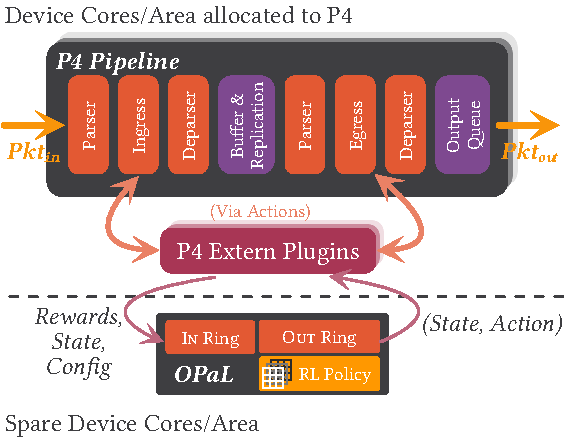
\includegraphics[keepaspectratio, width=0.75\linewidth]{figures/arch-with-p4}
	\caption{\approachshort{} brings low-latency, online reinforcement learning directly to the dataplane. SoC- and NetFPGA-based SmartNIC devices expose spare compute---making in-situ, asynchronous processing and learning possible alongside P4 dataplanes. Classical RL policy methods are the key to making this computationally feasible.\label{fig:netro-arch}}
\end{figure}
Automatic network optimisation, control, and defence are at last becoming commonplace.
Adaptive techniques such as \emph{reinforcement learning} (RL) have led the charge in data-driven networking, enhancing automatic traffic/media optimisation~\parencite{DBLP:conf/sigcomm/ChenL0L18,DBLP:conf/sigcomm/MaoNA17}, congestion control~\parencite{DBLP:journals/corr/abs-1910-04054}, adaptive routing~\parencite{DBLP:conf/hotnets/ValadarskySST17,DBLP:conf/conext/GiladSGRS20}, resource management~\parencite{DBLP:conf/hotnets/MaoAMK16}, and packet classification~\parencite{DBLP:conf/sigcomm/LiangZJS19}.
In RL methods, every change and its effects improve future decisions made by an agent.

%Parallel to this, P4~\parencite{DBLP:journals/ccr/BosshartDGIMRSTVVW14} and programmable dataplane hardware~\parencite{DBLP:journals/micro/ZilbermanACM14, netronome-smartnic, xilinx-alveo, barefoot-intel} have inspired explosive growth and interest in the research community surrounding in-network computation and offloading.
%This has manifested in novel uses of programmable dataplane hardware to accelerate distributed tasks, fine-grained traffic measurement~\parencite{DBLP:conf/sigcomm/GuptaHCFRW18,DBLP:conf/sigcomm/ChenFKRR18,DBLP:conf/sosr/GhasemiBR17}, or per-packet processing.
%The latter is particularly attractive due to the costs of offloading to commodity host machines; input data must cross the PCIe bus several times, throughput requirements often impose the use of batching, and dedicated accelerators must again be contacted over PCIe~\parencite{DBLP:journals/corr/abs-2009-02353}.
%Additionally, in multi-tenant environments, IOMMU contention for both NICs and inference accelerators may impact tail latencies~\parencite{DBLP:conf/sigcomm/NeugebauerAZAL018}.
%In response, we have seen non-neural ML techniques~\parencite{DBLP:conf/hotnets/XiongZ19}, neural networks~\parencite{DBLP:conf/sigcomm/SanvitoSB18,DBLP:journals/corr/abs-1801-05731,DBLP:journals/corr/abs-2009-02353,langlet-ml-netronome}, and hardware design proposals for CGRA-based map-reduce blocks~\parencite{DBLP:journals/corr/abs-2002-08987} \emph{directly in the dataplane}.
%These works have shown the value in in-network ML: high-throughput, low latency response to network changes, particularly when co-hosted with state extraction.

%---

%?? Do we want concrete examples of things `pushed down the stack'?
%
%?? Consider a DDoS prevention system...
%?? in the face of new data, Able to start learning again in microseconds

In parallel, P4~\parencite{DBLP:journals/ccr/BosshartDGIMRSTVVW14} and \emph{programmable dataplane} (PDP) hardware~\parencite{DBLP:journals/micro/ZilbermanACM14, netronome-smartnic, xilinx-alveo, barefoot-intel} have inspired explosive growth and interest in the research community surrounding in-network computation and offloading.
The promise of PDP hardware is that we can move the entire monitoring and analysis stack \emph{into the dataplane itself, and have it evolve to incorporate new approaches}.
Consider a DDoS mitigation system which could react to dataplane-specific, per-packet state in microseconds, and \emph{start learning again just as quickly} in the face of new data or behaviours.
The P4 ecosystem already presents novel, openly-available, fine-grained traffic measurement techniques that can be installed and controlled with ease~\parencite{DBLP:conf/sigcomm/GuptaHCFRW18,DBLP:conf/sigcomm/ChenFKRR18,DBLP:conf/sosr/GhasemiBR17}.
In addition, P4's control plane makes it easy to select which flows or packets are monitored in a live network and potentially allow control over traffic at the decision site.
As a result, there has been keen interest in executing ML in the dataplane~\parencite{DBLP:conf/hotnets/XiongZ19,DBLP:conf/sigcomm/SanvitoSB18,DBLP:journals/corr/abs-1801-05731,DBLP:journals/corr/abs-2009-02353,langlet-ml-netronome,DBLP:journals/corr/abs-2002-08987} to take advantage of flow or per-packet state that cannot be efficiently processed or extracted at any other location in the network.
These works have shown the value of in-network ML: high-throughput, low latency response to network changes.
While they can exploit on-device state to provide reactive insight, the missing piece of the puzzle is learning and updating these ML analyses online without deferring to another machine in the network.
Training these models online and in-network is an exciting (and challenging) lacuna in the field that \emph{has yet to be addressed by the community}.

It is important to make this feasible, as offloading learning to commodity machines adds PCIe delays~\parencite{DBLP:journals/corr/abs-2009-02353,DBLP:conf/sigcomm/NeugebauerAZAL018}, but is required due to the complexity of modern ML.
For context, \emph{Deep Neural Network} (DNN) training relies on the backpropagation algorithm to compute gradients, can take vast amounts of offline simulation for RL~\parencite{DBLP:journals/corr/abs-1912-06680}, and needs many mini-batches of data for stable training.
These lead to high compute and storage costs, inducing capital expenditure for dedicated accelerators.
Moreover, high latencies \emph{caused} by offloading and expensive inference harm the learning process~\parencite{DBLP:journals/firai/TravnikMSP18} and impact runtime application performance~\parencite{DBLP:journals/corr/abs-1910-04054}.
If we can bring online learning \emph{to the dataplane}, then we can take advantage of rich, local state while minimising these latencies (and their impact on the learned policy).
This would also make it easy to train and prototype agent designs which can learn \emph{as the environment evolves}, or when there is too little data to model and simulate a problem.

%Moreover, DNN-backed RL must often be trained by vast amounts of offline simulation~\parencite{DBLP:journals/corr/abs-1912-06680}---in some cases compute-years worth~\parencite{DBLP:journals/corr/abs-1912-06680}---which can be counter-productive if the target problem evolves over time or is hard to model.

%?? rich, local state


%?? Why important to make feasible?
%?? Why horrid that it hasn't been looked at?
%This induces capital expenditure on 
%?? We focus on models \& methods to enable this

To enable \emph{online in-NIC learning}, we return to \emph{classical} RL methods and models.
In particular, we focus on tile-coding with one-step temporal-difference learning algorithms such as Sarsa.
%These choices have important benefits for in-NIC execution.
These functions do not require batches of inputs to learn in a stable way, negating the memory needed to store experience replays, and have simple update and inference logic.
Tile-coding in particular admits many optimisations, being an embarrassingly parallel problem.
Using fixed-point arithmetic, we solve the lack of floating-point support in PDP hardware \emph{and} enable new optimisations.
Moreover, the P4 dataplane can offer runtime control over which flows/packets are monitored.
%Finally, the choice of single-step algorithms (as opposed to $n$-step or Monte Carlo methods) bounds the amount of per-trace state required for online learning to just the last state-action pair, safeguarding the limited memory of the target devices.
We also design our solution to operate as closely as possible to the P4 pipeline to use and learn from per-packet state, but outside of the main packet path to prevent packet stalls.

%However, the task of \emph{training} these models online \emph{and} in-network presents an exciting (and challenging) lacuna in the field.
%Online training is particularly important if an agent needs to react to unforeseen (failure) states, such as in DDoS/intrusion prevention.
%For context, \emph{Deep Neural Network} (DNN) training relies upon the backpropagation algorithm to compute gradients, and for sizeable amounts of data to be held in mini-batches for stable training.
%Moreover, DNN-backed RL must often be trained by vast amounts of offline simulation---in some cases compute-years worth~\parencite{DBLP:journals/corr/abs-1912-06680}---which can be counter-productive if the target problem evolves over time or is hard to model.
%These space and compute requirements, at present, mandate that training must occur in commodity hosts or dedicated hardware.
%Moreover, high state-action latencies \emph{caused} by offloading and expensive policy approximations add significant noise to the learning process~\parencite{DBLP:journals/firai/TravnikMSP18} and impact application performance~\parencite{DBLP:journals/corr/abs-1910-04054}.

%?? Why programmable vs fixed dataplane?
%?? Entire monitoring and analysis stack in one device
%?? Why p4? Exploit existing works to get local state (and future works), Ease of runtime reconfig, control over traffic at the decision site.

%?? The chance to exploit 

%?? Emphasise related work claims here!
%?? We're doing novel stuff because ...



%?? quick, reactive insight

%?? without the capex on expensive, powerful hosts

The question we investigate is: can online RL be brought to the dataplane by returning to these computationally simpler methods, to act on locally extracted state?
Can it be made more efficient \emph{by dataplane hardware}?
Through this work, \approachshort{}, we can comfortably answer ``yes'' on both counts.
In particular, we exploit how SmartNIC devices often expose general-purpose compute to provide path-adjacent, on-chip RL in the dataplane (\cref{fig:netro-arch}).
As many of these devices have engineering and development histories which predate P4, general compute beyond P4's limits~\parencite{p4-psa} is surprisingly common.
By executing on spare compute units, we prevent packet stalling and offer quick runtime reconfigurability.
%We look backwards to classical RL techniques (tile-coded policies, single-step RL algorithms), alongside the adaptations introduced by existing in-network ML (such as quantisation).
%Such adaptations unlock further improvements in parallel inference and update processing.
This paper contributes:
\begin{itemize}
	\item An analysis of why in-NIC RL is needed and best-placed to interact with the network, made feasible by classical RL methods and quantisation (\cref{sec:motivation}),
	\item \emph{\approachshort{}}: a general-purpose in-NIC RL agent which scales with allocated device resources to meet latency or throughput demands of network traffic analysis (\cref{sec:design}),
	\item \emph{ParSa}, a wait-free, parallel, online RL algorithm to accelerate tile-coded policy inference and updates (\cref{alg:parsa}),
	\item In-depth evaluation of how \approachshort{} affects carried dataplane traffic, performs under different policy sizes (simple/complex state), and improves on explicit offloading with a \SI{15}{$\times$} latency reduction compared to commodity hardware (\SI{21}{$\times$} for 99.99\nthscript{th} tail latencies) and an order of magnitude improvement in online throughput (\cref{sec:evaluation}).
	\item A demonstration of how \approachshort{} would integrate with state-of-the-art PDP applications to perform fully in-NIC, fast, automated DDoS mitigation (\cref{sec:potential-integrations}).
\end{itemize}


%Automatic optimisation, control, and defence of networks are at last becoming commonplace.
%Data-driven networking has led the charge in traffic optimisation, congestion control and packet classification via adaptive techniques such as \emph{reinforcement learning} (RL), where every change and its measured effects further improve future decisions.
%Considering that the network evolves in its use and deployed protocols, this flexibility is essential.
%Yet data-driven methods suffer from a key weakness: they are dependent on both the recency and accuracy of input state.
%An out-of-date view of the world will lead to suboptimal choices, as will long processing times.
%These can result in worse performance and slower adaptation to the evolving network.
%
%Programmable dataplanes and in-switch compute, then, hold promise for integrating these new techniques in a feasible and efficient manner (beyond dedicated servers or virtualised network functions). For RL, key tasks include policy evaluation, online training, state collection, and action execution -- each of these introduces some degree of sensitivity to state accuracy. Ideally then, all logic would run on these programmable devices. Yet, there is often a finite budget in microcode/FPGA space, per-packet processing times, and available cores for execution. Moreover, necessary hardware, such as floating-point units, is unavailable in almost all cases.
%
%The precise costs and trade-offs which operators and designers must make have yet to be identified. This follows from a design space explosion induced by many necessary workarounds. For instance, quantisation or fixed-point arithmetic will allow training and control on all devices, but introduces further questions: what degree of quantisation is most appropriate? What effect would this have on training accuracy, communications cost, or storage requirements? More concerns arise when we consider core allocation, local vs. distributed training, and reliable lightweight communication in multi-agent scenarios. In all cases, network operators will not consider tools which affect underlying traffic.
%
%I aim to examine the effects of these choices on an existing RL-based DDoS attack mitigation system. To protect legitimate traffic, this controls packet drop and filtering for each flow using individual metrics observed by RL agents at ingress routers, and load measurements from several points along the path taken by the flow in question. The examined metrics include the throughput and latency of its individual components alongside system metrics: flow arrival-to-judgement time, and knowledge propagation time. Beyond this, it's crucial to identify what we can implement on pure P4-capable hardware. While extensions to P4 are fairly common in commodity hardware, the need for full design access (as in NetFPGA) or Micro-C (as in Netronome SmartNICs) represent a break from the clean, loop-free semantics of P4. As the market matures, these may represent different feature classes and price points.
%
%I will discuss early development efforts (including challenges and results) on the Netronome Agilio SmartNIC, which supports the P4 language as well as some degree of arbitrary microcode. I intend to present how reinforcement learning execution and network telemetry will differ in the above metrics when compared to a vNF-based deployment (i.e., software on external commodity servers).

\section{Preliminaries: RL for in-network computation}\label{sec:motivation}
We discuss recent trends in programmable switch hardware.
By combining this with insights from the ML/RL communities (past and present), we discuss why in-NIC RL is best-placed to interact with the network, and how classical RL methods and quantisation ensure computational feasibility.

Crucially, we train our focus on devices with a low port density, such as SmartNICs and the NetFPGA.
The designs of these devices make it reasonable to move policy processing \emph{outside of the packet pipeline}; SmartNICs expose many additional programmable cores, and NetFPGAs allow for the synthesis of independent functional units.
The main benefit of doing so is that core control logic can be moved as close to the device as possible \emph{without impacting packet processing rates}.
%?? Say more directly why this mode of operation is preferable to in-pipeline w/ P4
As ethernet moves beyond \SIlist{40;100}{\giga\bit\per\second}, packet processing deadlines grow tighter in tandem; a \SI{64}{\byte} packet must be produced every \SI{12.8}{\nano\second}, giving a \SI{3.99}{\micro\second} deadline on Netronome SmartNICs (having \num{312} P4 pipelines).
In-pipeline execution thus increases the risk of drops or stalled packet transmissions.

%However, this requires that there be a reasonably consistent interface and behaviour between device classes.
%This need for consistency underpins the \emph{Programmable Switch Architecture} (PSA)~\parencite{p4-psa}, which defines a conceptual model of match-action tables divided into ingress and egress pipelines.
%The PSA presents a sensible lower bound on the device capabilities required to implement a P4 dataplane, but the reality is more complex and interesting.

%?? TODO: trim down. Too ``thesis-y'', rather than ``conference-y''.
%?? Save this elsewhere 'til then?

\subsection{Programmable hardware capabilities}
%The introduction of the P4 language~\parencite{DBLP:journals/ccr/BosshartDGIMRSTVVW14} has led to explosive growth in the research community surrounding in-network computation and offloading.
%Providing a single language which is compatible with network devices of many form factors has been instrumental in the development of novel fine-grained traffic measurement approaches~\parencite{DBLP:conf/sigcomm/GuptaHCFRW18,DBLP:conf/sigcomm/ChenFKRR18,DBLP:conf/sosr/GhasemiBR17}.
%However, this requires that there be a reasonably consistent interface and behaviour between device classes.
%This need for consistency underpins the \emph{Programmable Switch Architecture} (PSA)~\parencite{p4-psa}, which defines a conceptual model of match-action tables divided into ingress and egress pipelines.
%The PSA presents a sensible lower bound on the device capabilities required to implement a P4 dataplane, but the reality is more complex and interesting.


%We would be remiss to believe that P4 and the PSA define all capabilities that programmable hardware supports.
%Many compatible devices have legacies long predating these developments. 
%For instance, many-core SOC-based Netronome SmartNIC~\parencite{netronome-smartnic}, and NetFPGA SUME~\parencite{DBLP:journals/micro/ZilbermanACM14} NICs allow virtually arbitrary programs to be specified and executed.
%The first of these compiles from P4$\rightarrow$Micro-C$\rightarrow$bytecode (with Micro-C externs), while the latter can combine the P4$\rightarrow$NetFPGA toolchain~\parencite{DBLP:conf/fpga/IbanezBMZ19} with arbitrary circuit externs---both exposing further device capabilities beyond the specification.
%This pattern extends to other SmartNICs, such as NVIDIA BlueField~\parencite{nvidia-bluefield} and Xilinx Alveo~\parencite{xilinx-alveo} devices.

While the P4 language~\parencite{DBLP:journals/ccr/BosshartDGIMRSTVVW14} has led to great interest in network programmability, it requires similar behaviour between device classes.
This is encoded as the \emph{Programmable Switch Architecture} (PSA)~\parencite{p4-psa}---a sensible lower bound on the device capabilities required to implement a P4 dataplane.
We would be remiss to believe that P4 and the PSA define all capabilities that programmable hardware supports.
Many compatible devices have legacies long predating these developments. 
For instance, many-core SOC-based Netronome~\parencite{netronome-smartnic}, NetFPGA SUME~\parencite{DBLP:journals/micro/ZilbermanACM14,DBLP:conf/fpga/IbanezBMZ19}, and other SmartNICs~\parencite{nvidia-bluefield,xilinx-alveo} allow virtually arbitrary programs to be specified and executed.
%This pattern extends to other SmartNICs~\parencite{nvidia-bluefield,xilinx-alveo}.

Currently, low port density devices like the above are most likely to have specific general-purpose compute, as they are designed to suit high-performance offloading and middlebox development.
Even Intel Tofino~\parencite{barefoot-intel} ASICs, which architecturally mirror the PSA, expose additional matching capabilities and \emph{arithmetic logic unit} (ALU) functions via the Tofino Native Architecture.
Regardless, floating-point operations key to ML/RL workloads are very rarely supported outside of deep learning accelerators (which, in turn, lack packet switching functionality).
Moreover, the limited memory/block RAM and per-packet timing constraints endemic to these devices make this class of in-NIC offloading challenging.

%\begin{insight}
%	Current low-port density programmable network devices often have spare resources and extra capabilities beyond the PSA specification which can aid asynchronous, local compute.
%\end{insight}

\subsection{Reinforcement Learning}
%\emph{Reinforcement learning} (RL) algorithms are methods of training an \emph{agent} to choose an optimal sequence of actions in pursuit of a given task \cite{RL2E}.
%Like most machine learning methods, an RL algorithm uses gradient information to update the parameters used to approximate a function.
%In RL contexts, this is a state$\rightarrow$action function known as a \emph{policy}.
%When training, agents are given \emph{reward measurements} and a learned policy acts to maximise the \emph{expected discounted reward} received.
%When a pre-trained policy is deployed, this signal is not required.
%
%It's useful to consider how these algorithms differ from other ML use cases, such as classifiers.
%The main differences lie in how this gradient information is used, and combined with \emph{reward measurements} received from the environment.
%Rather than adapting the learned parameters along the gradient using an error value from a target value, because the optimal actions aren't known they adjust values using a \emph{Markov Decision Process} (MDP)---capturing state trajectories to adjust value based on past and future decisions.

\emph{Reinforcement learning} (RL) algorithms train an \emph{agent} to choose an optimal sequence of actions in pursuit of a given task~\parencite{RL2E}.
Like most ML methods, RL algorithms use gradient information to update the parameters used to approximate a function with \emph{reward measurements} from the environment.
RL's \emph{Markov Decision Process} (MDP) structure allows online learning of a state-action map in a model-free way, and can step through local minima when needed compared to ML.
In networking, this allows for learning to respond to on-device state or to handle rapidly evolving problems.
RL algorithms are generally agnostic to the policy approximation used, and classical single-step methods are simple---most of the compute work is occupied by the policy itself.
Consider the single-step, semi-gradient Sarsa algorithm~\cite[pp. \numrange{217}{221}]{RL2E} which requires only additions and multiplication to update and learn a policy online.

%Consider the single-step, semi-gradient Sarsa algorithm~\cite[pp. \numrange{217}{221}]{RL2E}:
%\begin{subequations}
%	\begin{gather}
%		\delta_t = R_{t+1} + \gamma \acval{S_{t+1}}{A_{t+1}}{\wvec{t}} - \acval{S_t}{A_t}{\wvec{t}},\\
%		\bm{w}_{t+1} = \bm{w}_{t} + \alpha \delta_t \nabla{\acval{S_t}{A_t}{\wvec{t}}},
%	\end{gather}%
%	\label{eqn:sg-sarsa}%
%	where $\delta_t$ is known as the \emph{temporal-difference} (TD) error, $\acval{S}{A}{\wvec{}}$ denotes the \emph{value} of an action $A$ taken in state $S$ according to the policy $\wvec{}$, and the vector gradient $\nabla$ is taken with respect to $\wvec{}$. $\gamma,\alpha\in[0,1]$ are the discount factor and learning rate (governing the degree of forward planning and policy stability, respectively).
%\end{subequations}
%In essence, at each timestep the policy parameters ($\wvec{}$) are increased along the gradient ($\nabla{\acvalblank}$) using a fixed learning rate ($\alpha$) and a computed adjustment ($\delta_t$).
%This adjustment is equal to the difference between the chosen action $A$'s value in state $S$ and the reward received ($R_{t+1} - \acval{S_t}{A_t}{\wvec{}}$), \emph{plus} some part of the \emph{next} action's value ($\gamma\acval{S_{t+1}}{A_{t+1}}{\wvec{}}$).
%To give some context on the design space here, other algorithms may employ separate state value approximations, use the entirety of an agent's trace, or be tailored to characteristics of the policy approximator (e.g., how neural networks benefit from batching).

%\begin{insight}
%	Classical, single-step RL algorithms are computationally simple and are agnostic to the policy approximation used. Furthermore, they require only additions and multiplication to update and learn a policy online.
%\end{insight}

\fakepara{RL in asynchronous environments}
%There remains some degree of divergence between the theory and implementation of RL agents.
%Consider \cref{fig:state-slip}: the traditional formulation of a Markov decision process assumes that an agent receives a new view of the world's state at fixed time intervals, and then decides upon and executes an action instantly.
%The reality is that state information takes time to traverse the network, service times are offset by how quickly hosts respond to interrupts and deserialise requests, and action preference lists are often computed via expensive policy approximations.
%Action installation also incurs costs in fields such as network administration, initially to contact the controller and then for those actions to be installed via the control plane.
Consider \cref{fig:state-slip}: the traditional RL formulation assumes that an agent receives new state at fixed time intervals, and then decides upon an action instantly, while in reality these incur transmission and compute delays.
This adds noise to the state-action mapping being learned, which has harms learning rate and final accuracy even for simple grid world tasks~\parencite{DBLP:journals/firai/TravnikMSP18}.
Reordering algorithmic steps reduces these costs for online single-step algorithms, but reducing this further requires detailed agent-environment co-design.
This principle has influenced the design of real network use cases, such RL-based congestion-control algorithms~\parencite{DBLP:journals/corr/abs-1910-04054}, showing that asynchrony is necessary for high-speed applications.
This often requires that state measurements are fused~\parencite{DBLP:journals/corr/abs-1910-04054,DBLP:journals/tnsm/SimpsonRP20} while expensive computations are ongoing.
`Stopping the world' causes significant performance degradation, as inference takes up to \SI{30}{\milli\second} in the above work on congestion control, or any time-sensitive control problems.

\begin{figure}
	\begin{subfigure}{0.45\linewidth}
		\centering
		\resizebox{0.9\linewidth}{!}{
			\centering
			\begin{tikzpicture}
				\node[circle, draw] (state) {$S$};
				\node[circle, draw] (state') at ($(state) + (0, -2)$) {$S'$};
				
				\node (agent) at ($(2, 0) + (state)$) {Agent};
				\node[below of=agent] (action) {Action $A$};
				
				\node[right of=state'] {$+ R$};
				
				\draw[->] (state) -- (state') node[midway, right] {$A$};
				
				\draw[dotted, ->, bend left = 30] (state) -- (agent);
				\draw[->] (agent) -- (action);
				\draw[dotted, ->] (action) -- (state);
		\end{tikzpicture}}
		\caption{Theory: state measurement, action computation, and learning are zero-cost.}
	\end{subfigure}
	\hspace{0.05\linewidth}
	\begin{subfigure}{0.45\linewidth}
		\centering
		\resizebox{0.7\linewidth}{!}{
			\centering
			\begin{tikzpicture}
				\node[circle, draw] (state) {$S$};
				\node[circle, draw] (state') at ($(state) + (0, -1.5)$) {$S'$};
				\node[circle, draw] (state'') at ($(state') + (0, -1.5)$) {$S''$};
				
				\node (agent) at ($(2, 0) + (state)$) {Agent};
				\node[below of=agent] (action) {Action $A$};
				
				\node[right of=state''] {$+ R$};
				
				\draw[->] (state) -- (state') node[midway, right] {$\varnothing$};
				\draw[->] (state') -- (state'') node[midway, right] {$A$};
				
				\draw[dotted, ->, bend left = 30] (state) -- (agent) node[midway, above] {$t_1$};
				\draw[->] (agent) -- (action) node[midway, right] {$t_2$};
				\draw[dotted, ->] (action) -- (state') node[midway, below] {$t_3$};
		\end{tikzpicture}}
		\caption{Reality: costs of measurement and action lead to \emph{state drift}---over a time delay $t_1+t_2+t_3$, inaction transforms state $S$ into $S'$.}
	\end{subfigure}
	\caption{Asynchronous RL delays and state slippage.\label{fig:state-slip}}
\end{figure}

%?? Find some cites citing the relevance of this problem wrt. self-driving cars, robotics, etc.

This cost is what drives us to \emph{bring online reinforcement learning to the dataplane}---referring again to \cref{fig:state-slip}, we would place P4-based state measurement ($t_1$), simple policy approximation ($t_2$), and controlled systems ($t_3$) as close to one another as possible.
In networks, actions are most likely to be installed on backbone switches, bump-in-the-wire NICs or middleboxes, and in the NICs of end-hosts---all of which make in-NIC training a perfect fit.
As such, our goal is to collocate \emph{all} functions which comprise an RL agent on the same chip or device.
Both programmable devices and the network environment make this more difficult, as we'll examine in the sequel.

%?? Return to dimitris note: how is this important to final solution?

%\begin{insight}
%	Online control problems benefit from low-latency, local execution and training (i.e., in-NIC/switch).
%\end{insight}

\subsection{Efficient policy approximation}
%Some problems either evolve over time in unpredictable ways, or cannot be easily modelled.
%This can then make \emph{online} learning of the task an attractive prospect, using a single available stream of experience.
%\emph{Deep neural networks} (DNNs), particularly when used as the basis for an RL agent's policy, require vast amounts of experience to converge on an accurate parameter set.
%In many problem domains, this equates to training from compute-years worth of distributed offline simulations, which is at odds with the need to adapt to changes in the underlying problem \emph{as they happen}.
%Achieving stable learning requires sizeable batches of gradients to be computed, potentially using the entire experience replay from each simulation.
%Although there has been a vested interest in efficiently \emph{executing} more complex function approximators such as DNNs in-NIC~\parencite{DBLP:journals/corr/abs-2002-08987,DBLP:journals/corr/abs-2009-02353,DBLP:conf/sigcomm/SanvitoSB18,DBLP:journals/corr/abs-1801-05731,langlet-ml-netronome}, the computational cost of gradient computation via backpropagation remains too significant on embedded hardware.
Complex \emph{Deep Neural Networks} (DNNs), particularly when used as the basis for an RL agent's policy, require vast amounts (e.g., in the worst case compute-years~\parencite{DBLP:journals/corr/abs-1912-06680}) of experience to converge on an accurate parameter set, which is at odds with the need to adapt to changes in the underlying problem \emph{as they happen}.
Although there has been a vested interest in efficiently \emph{executing} complex function approximators like DNNs in-NIC~\parencite{DBLP:journals/corr/abs-2002-08987,DBLP:journals/corr/abs-2009-02353,DBLP:conf/sigcomm/SanvitoSB18,DBLP:journals/corr/abs-1801-05731,langlet-ml-netronome}, the storage and computational costs of backpropagation remain too significant on embedded hardware.

%?? Probably want some cites on the need for batching in NN methods, even though this is understood. DL book?

We return to what classical RL methods can offer us; in particular, the simple linear function approximation given by \emph{tile coding} \cite[pp.\ \numrange{217}{221}]{RL2E}.
The idea is simple: a policy is represented by sets of tiles, each covering one or more dimensions of the input state with several overlapping tilings (offset stepwise to provide generalisation).
This covers any input-output mapping, such as converting packet header data into a preference list for queue priorities.
A state vector produces a single `hit' in each tiling, all of which then correspond to a list of action preference lists.
Inference (choosing an action) is then simply summing over all such lists to obtian a final action preference list, selecting the maximum.
Updating at the next timestep uses this same list of lists, adjusting the value of the last selected action using a value $\delta_t$ computed through Sarsa.
Crucially, this internal representation ensures that there are no data dependencies between any tile calculations for an input.
This has important benefits for parallelising the key parts of an RL algorithm; both action selection and policy updates are map-reduce problems.
To select an action, we can produce a task for each tiling---retrieving the list of action values contributed by the tile activated by the input state.
An aggregate step sums up all action preference lists, and the action with the highest value is then selected.
Updating the policy (with a new $\delta_t$ value) has no aggregate step, and as tile indices map to disjoint memory regions no locks are required.
%As we show in \cref{sec:design}, it is possible to make the inference aggregate step wait-free.

For instance, a policy with $m$ sets of tiles (each having its own set of input dimensions), each containing $n$ overlapping tilings then creates $m \times n$ separate tasks.\footnote{Retrieving each individual action's value can be considered a work item (giving $m \times n \times a$ tasks when there are $a$ actions). However, this requires the tile coding operation to repeated $a$ times per tile, which is likely extremely wasteful outside of extreme degrees of parallelism.}
As an example, a real-world policy size which we examine later (\cref{sec:experimental-setup}) with one bias tile and \num{16} sets containing \num{8} tilings creates \num{129} work items.

Computing a tile hit requires one division per dimension, which is an expensive addition to the ALU operations we require from a platform.
However, if the width of tiles are fixed at powers-of-two, then these may be replaced with right bitshifts.
As we shall see shortly, this aligns with our choice of numerical representation.

%\begin{insight}
%	Tile coded policies are embarrassingly parallel in both inference \emph{and} learning. Moreover, in some instances the process can be altered to require only bitshifts, additions, and multiplication.
%\end{insight}

\subsection{Numerical representation for embedded ML}
A key feature universally lacking from PDP hardware is floating-point arithmetic support.
Luckily, the task of bringing ML models to resource-constrained environments without these capabilities is well-studied.
Quantisation and alternative data formats have been suggested to make ML inference feasible on resource- and power-limited platforms, work around hardware constraints, or compute faster and more efficiently.
Lower bit depths reduce memory footprints, and improve throughput in designs such as \emph{bfloat16}~\parencite{bfloat16-blog} in Google TPUs~\parencite{DBLP:journals/sigops/XieDMKVZT18}, \emph{hfp8}~\parencite{DBLP:conf/nips/SunCCWVSCZG19}, and other floating point formats~\parencite{DBLP:journals/corr/abs-2007-01530}.
In many cases, accuracy losses for doing so are negligible.
Much of this work goes further still towards integer~\parencite{tensorrt-8bit} or binarised~\parencite{DBLP:journals/corr/MiyashitaLM16,DBLP:conf/eccv/RastegariORF16,DBLP:journals/corr/KimS16,DBLP:conf/nips/HubaraCSEB16} representations, sacrificing dynamic range for simpler arithmetic operations.
The works mentioned above use similar techniques to make inference tractable on network hardware, i.e., to bring neural networks to the dataplane~\parencite{DBLP:journals/corr/abs-2009-02353,DBLP:conf/sigcomm/SanvitoSB18,DBLP:journals/corr/abs-1801-05731}.

To make RL workloads feasible under such constraints, we propose the use of quantised, fixed-point representations such as $Qm.n$ (i.e., $m$\si{bit} signed integers with an $n$\si{bit} fractional part), which allow us to evaluate and update policies using only integer arithmetic.
This is not only essential in performing this work, but also serves as a mechanism for reducing the processing and memory costs of function approximation.
We note that our later parallel, wait-free Sarsa implementation---\emph{ParSa} (\cref{alg:parsa})---is possible only due to the use of $Qm.n$, as atomic operations on floating point numbers typically do not exist outside of graphics-processing hardware.

%When combined with the above P4-driven techniques for in-network flow/device measurement, we at last have the mechanisms to collocate the key processes of an RL agent.
%Moreover, the base P4 dataplane can be used to simplify parsing logic and offer runtime control over which flows/packets are monitored, alongside other packet actions.
%This again fits our goals of integrating RL techniques directly within bump-in-the-wire installations and at end-hosts.

%\begin{insight}
%	Fixed point quantisation allows us to perform numerical calculations using only integer arithmetic.
%	Existing literature to-date supports the effectiveness and use of these techniques on embedded ML deployments.
%\end{insight}

%\subsection{Netronome Platform Fundamentals}
%As we implement this work on Netronome SmartNICs (thus the NFP chip architecture), it is necessary to explain its basics.
%NFP chips are \emph{system-on-a-chip} (SoC) devices, and achieve scalable packet processing through sheer parallelism.
%Aside from an ARM management chip and application specific functional units, most of the chip is composed of \emph{microengines} (MEs), grouped into \emph{islands} of 4 or 12 MEs.
%All 12-ME islands are used by a default P4 pipeline.
%Each ME has \numrange{4}{8} \emph{contexts} (hardware threads) which share a code store and large register file, offering zero-cost context switches triggered by I/O.
%Contexts and MEs may send one another numbered signals, and MEs have a small \emph{next-neighbour} register file for passing values in one direction to the next ME on the same island.
%MEs run a proprietary instruction set, compiled to via a \emph{(Micro-)C} compiler.
%Beyond registers, the platform implements an explicit memory hierarchy scaling in size, location, and access cost as below:
%$$\text{LMEM (ME)} < \text{CLS (Island)} < \text{CTM} < \text{IMEM (Chip)} < \text{EMEM}$$

\section{Design and Implementation}\label{sec:design}
Based on the design principles, problems, and potential solutions outlined throughout \cref{sec:motivation}, we present our design for an in-NIC, task-independent, online reinforcement learning system---\emph{\approachshort{} (\approach)}.
At a high level, \approachshort{} is designed to use the auxiliary compute exposed by general SmartNIC devices to offer low-latency online learning, scaling according to available on-chip resources at build time.
As the allocation of cores/chip area is set ahead of time by a framework or system administrator, \approachshort{} (\Coopfw) agents enumerate themselves at runtime initialisation.

\begin{figure*}
	\centering
	\begin{subfigure}{0.45\linewidth}
		\centering
		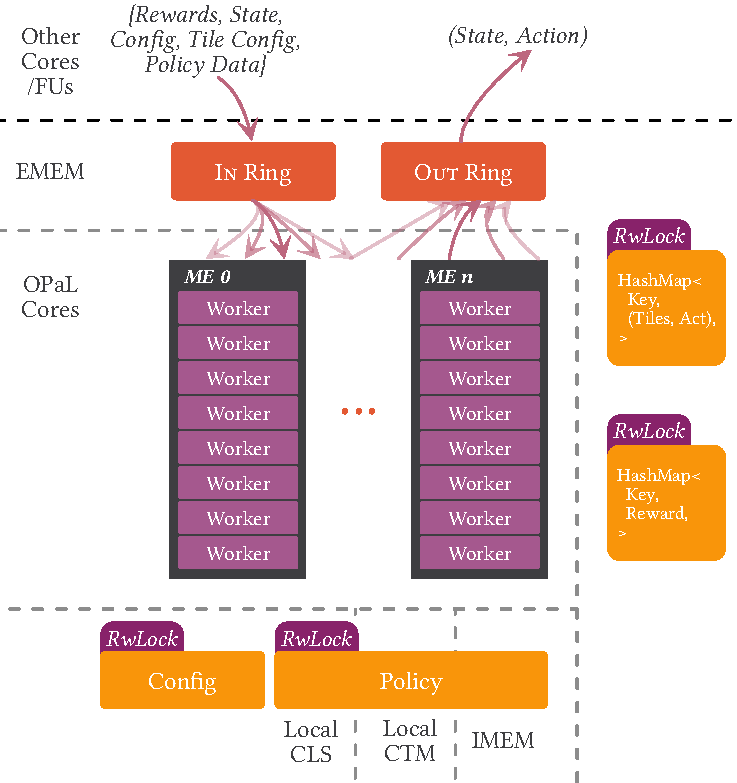
\includegraphics[keepaspectratio, width=0.85\linewidth]{figures/ind}
		\caption{\Indfw{} (offline throughput-optimal). \emph{Workers} independently pull commands from (and push state-action pairs to) the environment, locking access to the policy when updates must occur.\label{fig:single-and-parallel:single}}
	\end{subfigure}
	\hspace{0.04\linewidth}
	\begin{subfigure}{0.45\linewidth}
		\centering
		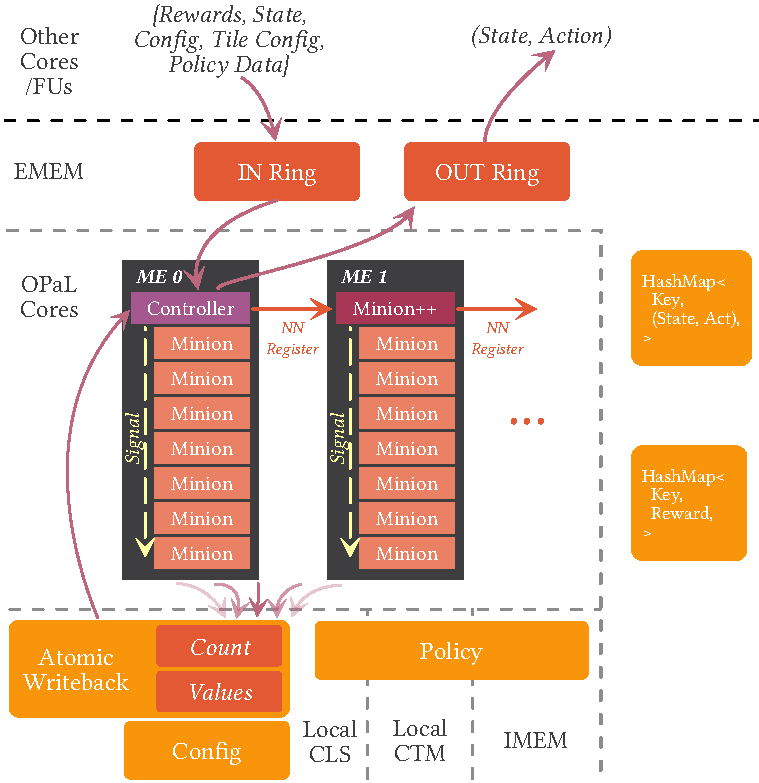
\includegraphics[keepaspectratio, width=0.85\linewidth]{figures/coop}
		\caption{\Coopfw{} (online-optimal). A single \emph{controller} delegates RL computation and updates to many \emph{minion} threads, who operate on independent subtasks.\label{fig:single-and-parallel:parallel}}
	\end{subfigure}
	\caption{\approachshort{}'s compute strategies scale to fit device capacity according to either latency or throughput needs.\label{fig:single-and-parallel}}
\end{figure*}

\Cref{fig:netro-arch,fig:single-and-parallel} outline our design and implementation on Netronome SmartNIC hardware in pursuit of this goal: unused device resources beyond the P4-PSA spec \emph{can and should be used} to drive asynchronous environmental control.
We explain relevant NFP architectural details in \cref{sec:netronome-platform-fundamentals}.
\approachshort{} communicates with the packet pipeline of a P4 dataplane via \texttt{extern} plugins using \inring{} (state, configuration) and \outring{} (action) messages (\cref{fig:netro-arch}).
Internally, \approachshort{} either has all its cores act independently (\cref{fig:single-and-parallel:single}) or cooperate to solve each task (\cref{fig:single-and-parallel:parallel})---with different latency-throughput benefits (\cref{sec:action-and-update-computation}).
We open-source our firmware design and control programs for the benefit of the community.\footnote{\textanon{\url{https://github.com/FelixMcFelix/pdp-rl-paper}}{Link redacted for double-blind submission.}}
Moving beyond the Netronome platform, we describe how our architectural choices may be adapted and improved upon by more bespoke hardware or FPGA-based deployment.

\subsection{System Model}
\approachshort{} is a general, task-independent framework for in-network, online training and execution of \emph{any reinforcement learning agent design} using classical methods.
\approachshort{} is agnostic to the meaning of state vectors it receives as inputs and the actions it produces, which are employed by other functional units or the dataplane.
However, in-NIC/in-network execution specifically benefits packet-, flow-, and network-level learning, control, and optimisation tasks.

\approachshort{} runs on one or more cores of a SmartNIC to convert fixed-point state measurements from the environment into a stream of actions using a stored policy.
As an example, this might be to map flow state and performance measurements into a queueing priority for future packets from that flow, or to compute and apply a rate limit to preserve quality of service.
These dedicated cores are then responsible for processing requests, computing actions, and updating the underlying policy in real time.
Combined with reward measurements, this policy can then be updated or trained from scratch entirely on the NIC, acting as a fully online RL agent.
An input state vector \emph{always} induces an action and, if desired, updates the policy using either an included reward or one retrieved from memory according to a (configurable) key placed alongside the state.
This allows for simultaneous control and learning over independent systems by the same agent (i.e., optimising several flows with their own reward measures, such as DDoS mitigation in an AS where each next-hop AS might have their own `health' metric).

%However, high-speed data networks impose inviolable per-packet deadlines.

To protect traffic throughput and allow for effective deployment in as many environments as possible, \approachshort{} places RL execution on-chip, \emph{but off the main packet path}, communicating and running parallel to the main P4 dataplane.
As shown in \cref{fig:netro-arch}, this asynchrony allows coexistence with P4 programs, and imposes minimal impact on carried traffic for both bump-in-the-wire deployments and at end-points.
For instance, in the default deployment of a P4 packet processing pipeline on Netronome NFP chips several of these cores go unused (as does spare area on an FPGA design), making this paradigm possible.

%The main interaction model is that platform-specific IPC (message rings) is used to \emph{push} configuration, state vectors, and reward measurements to the RL system.
%These same mechanisms are used by other cores on the same device to \emph{pull} output actions from the RL system.
%Both input and output can occur on any other core of the device, i.e., as part of P4 \texttt{extern} plugins or a dedicated flow state measurement subsystem, while the P4 control plane itself provides granular control over which flows are monitored or affected.
%
%Runtime reconfiguration and interaction occur via the control and/or dataplane: the ease of use of the P4 pipeline's match-action tables and custom protocol parsers, combined with the dedicated input pipe to the NIC's controller (the host machine), allow these to be cleanly separated or combined as needed.
%Bit depth of quantised measurements/preferences, maximum policy sizes, and parallelisation strategy may be configured at compile time.

\subsection{Action and Update Computation}\label{sec:action-and-update-computation}
\approachshort{} applies the insights of \textcite{DBLP:journals/firai/TravnikMSP18} to minimise action latency; an action is computed, sent out into the environment, and only then is the underlying policy updated.
Using one of the below strategies chosen at compile time, a state vector is tile coded, converted into action probabilities, and an action is chosen.
This is then written out to the environment as in \cref{sec:agent-environment-communication}.
If online learning is enabled, \approachshort{} then checks an internal hashmap for a previous state-action pair matching the current instruction source, and if found then the policy is updated.
Updates are computed using \emph{single-step semi-gradient Sarsa}~\cite[pp. \numrange{217}{221}]{RL2E}, though modification to support other single-step methods would be trivial.
The new state- or tiles-action pair is then written into storage.
\approachshort{} can be configured to automatically select values of the input state vector as keys for state and reward storage.

Two main firmware models govern how the computation-intensive parts of these tasks (tile-coding, action preference list construction, policy updates) are carried out:
\begin{description}
	\item[\Indfw{} (\cref{fig:single-and-parallel:single})] Separate threads listen for new states, and each performs its work sequentially. Computing an action list requires a \emph{read lock} on the policy. If an update occurs, the core requests a \emph{write lock} before updating, greatly limiting online throughput. \emph{Tile lists} are stored for update computation.
	\item[\Coopfw{} (\cref{fig:single-and-parallel:parallel,alg:parsa})] Threads cooperate on processing state vectors, minimising latency. \emph{Minions} have a fixed list of work items, while a \emph{controller} thread sends compute/update commands before awaiting worker completion. Work items are disjoint, requiring no policy locks. \emph{State vectors} are stored for update computation.
\end{description}
Each offers a different point of optimisation; if updates are disabled, then the \indfw{} model can maximise throughput, while the \coopfw{} model is designed to minimise decision latency and needs no locks for updating the policy (increasing \emph{online learning} throughput).
These correspond to only executing a trained policy and actively (re-)training a policy, respectively.
%ParSa is described here at a high level, as an algorithm suited for \emph{any multiprocessor environment}.
%We omit the simple logic for $\epsilon$-greedy action selection (which we implement), and note that modification to other single-step algorithms such as \emph{Q-learning} would be trivial.
%We detail our communication primitives in \cref{sec:intra-agent-communication}, and our work scheduling strategy in \cref{sec:work-allocation}, eliding the details of tile-coding as they are well-understood.
%In general it is also possible for the \emph{Ctl} task to act as an additional \emph{Minion} in its parallel sections; we were limited here by code store requirements on the NFP.
Latency and throughput, as in many networked systems, have different effects upon RL agents according to their design and target problem.
Higher RL throughput is a necessity for per-flow or per-packet applications, which can require high decision-per-second rates even after combining state measurements received from the environment, such as flow control in DDoS prevention.
Equally, lower latency affords an agent finer-grained control and learning of a problem, being able to react sooner to new information (e.g., device state in a routing optimisation problem, or queue depth when trying to enforce packet pacing).

Paradoxically, we found that in the general \emph{ParSa} algorithm it was more efficient \emph{to do more work} by having each worker recompute its tile subset from a stored state.
It transpired that cacheing this data placed a larger \texttt{memcpy} in the serial section, whose size did not scale at all with bit depth.
Additionally, we do not use bitshifts in place of division operations in our implementation, due to the strict limits that power-of-two tile widths place upon policy design.

\subsection{Agent-Environment Communication}\label{sec:agent-environment-communication}
\approachshort{} uses \emph{multiple-producer/multiple-consumer} (MPMC) messaging channels to communicate with other computational elements; be they P4 programs on the packet path, or additional on-chip analysis and control modules.
Through these channels the system \emph{pushes} state vectors, reward measures, and control/setup packets as its inputs, and \emph{pulls} a stream of state-action pairs as its outputs.
This allows decisions to be made asynchronously---preventing packet stalling---and allowing many parallel decision-making agents to be used if desired.
The key insight of this mechanism is that on-chip reward/state signals enjoy first-class support in the same manner as packets from the P4 dataplane, allowing agents to act on environmental signals from other on-NIC/chip asynchronous processes or the controller.
As such, \approachshort{} can receive from P4 \texttt{extern}s or another dedicated off-path flow state measurement application.

Our implementation uses platform-specific IPC (\emph{EMEM ring buffers}) with hardware signalling mechanisms on work arrival to achieve this.
As PDP hardware lacks dynamic memory allocation, P4 pipeline threads request buffers for packet payloads using a shared freelist to enable state/configuration/policy data handover.
Packet headers are extracted and parsed using the tooling autogenerated by the P4 pipeline.
We found that this costs a median \SIrange{126}{140}{\nano\second} communication time (local--remote), comparable to message channels in the Rust and Go languages on commodity hardware.

%The main interaction model is that platform-specific IPC (message rings) is used to \emph{push} configuration, state vectors, and reward measurements to the RL system.
%These same mechanisms are used by other cores on the same device to \emph{pull} output actions from the RL system.
%Both input and output can occur on any other core of the device, i.e., as part of P4 \texttt{extern} plugins or a dedicated flow state measurement subsystem, while the P4 control plane itself provides granular control over which flows are monitored or affected.

\subsection{Intra-Agent Communication}\label{sec:intra-agent-communication}
Even with parallel problems such as \emph{ParSa}, optimising for latency requires meticulous care in how work is passed out and aggregated.
This is truer still when moving from the moderately fine-grained control of classical RL methods ($\sim$\SI{1}{\milli\second}) to its logical limit (tens of \si{\micro\second}).
Ordinarily, the marshalling of requests, responses, and safe shared data access can incur significant extra overheads.
On-chip execution and the nature of action preference computation allow us to use lockless atomic aggregation, removing the overheads of explicit messaging/packetisation.
Moreover, physically adjacent functional units/cores often have special-purpose shared registers or share a small fast cache to accelerate communication.

%?? reduce below and make take-homes more generic if possible

Our implementation exploits the locality of cores in the NFP architecture, which can be used on other platforms like NetFPGA.
Policy compute/update/configure tasks are passed between cores using direct \emph{next neighbour} registers, signalling all child threads in response.
Such on-chip signals cost just $\sim$\SI{20}{\nano\second} per relayed message.
Each core performs atomic adds to a shared preference list and an acknowledgement counter checked by the master thread, implementing the wait-free \emph{ParSa} algorithm we introduce (\cref{alg:parsa}).
This is essential for aggregation compared to the use of bounded message buffers, which caused significant head-of-line blocking.

%On-chip local messages cost us just $\sim$\SI{20}{\nano\second} latency per relayed message
%
%In earlier designs we had experimented with bounded buffers as in \cref{sec:agent-environment-communication} for this, modified to be located solely in CLS memory, dedicating the master thread to result aggregation.
%We found that this created a performance bottleneck at this final stage, causing significant head-of-line blocking for each of the workers.
%Similarly, our next neighbour work notification scheme ($\sim$\SI{20}{\nano\second} latency per relayed message) was examined against \emph{reflector} and \emph{work queue} IPC mechanisms (\SIlist{58;126}{\nano\second} per messaged core).
%These slower messages can be used in theory to skip ahead into longer ME chains.

%Our implementation exploits the locality of threads, cores, and their parent islands in the NFP architecture.
%Policy compute/update tasks and configuration updates are passed between cores using these direct \emph{next neighbour} registers, signalling all child threads in response.
%Each task performs atomic adds to a shared preference list, and atomically increments an acknowledgement counter to be periodically checked by the master thread, implementing the wait-free \emph{ParSa} algorithm we introduce (\cref{alg:parsa}).

%In earlier designs we had experimented with bounded buffers as in \cref{sec:agent-environment-communication} for this, modified to be located solely in CLS memory, dedicating the master thread to result aggregation.
%We found that this created a performance bottleneck at this final stage, causing significant head-of-line blocking for each of the workers.
%Similarly, our next neighbour work notification scheme ($\sim$\SI{20}{\nano\second} latency per relayed message) was examined against \emph{reflector} and \emph{work queue} IPC mechanisms (\SIlist{58;126}{\nano\second} per messaged core).
%These slower messages can be used in theory to skip ahead into longer ME chains.

\begin{algorithm}
	\caption{ParSa---\emph{Par}allel \emph{Sa}rsa\label{alg:parsa}}
	\SetKw{Let}{let}
	\SetKw{Enum}{enum}
	\SetKw{In}{in}
	\SetKw{Await}{await}
	\SetKw{Const}{const}
	\SetKwProg{parsa}{Function \emph{ParSa}}{}{end}
	\SetKwProg{control}{Function \emph{Ctl}}{}{end}
	\SetKwProg{minion}{Function \emph{Minion}}{}{end}
	\SetKwProg{tilecode}{Function \emph{TileCode}}{}{end}
	
	\tcc{Given message passing mechanisms \emph{scatter} and \emph{recv}, quantised arithmetic functions $Q_\mathit{mul}$ and TileCode, and omitting schedule/config/precache updates.}
	\tcc{\emph{cfg}.$\alpha$, \emph{cfg}.$\gamma$ are hyperparameters affecting the significance of each update and the degree of forward-planning, respectively.}
	
	\Enum Par \{ Act(\emph{state}), Upd(\emph{delta, action, state}) \}\;
	\Const \emph{cfg, policy} = /* ... */\;
	
	\Let \emph{values}: [AtomicI32; cfg.n\_actions] = \{0\}\;
	\Let \emph{acks}: AtomicI32 = 0\;
	\parsa{id, schedule}{
		\uIf{id==0}{
			\ForAll{state\_pkt \In \inring{}}{
				Ctl(state\_pkt)\;
			}
		}
		\Else{
			\While{true}{Minion(schedule[id - 1], recv())\;}
		}
	}

	\control{state}{
		\emph{values, acks} = \{0\}, scatter(Par::Act(\emph{state}))\;
		acquire slot for \outring, copy \emph{state} into slot\;
		\Await acks == \emph{cfg.n\_minions}\;
		\Let \emph{action} = argmax(\emph{values})\;
		write \emph{action} into \outring{} slot, enqueue\;
		\If{cfg.online}{
			\Let \emph{((l\_state, l\_act, l\_val), found\_s)} = \emph{cfg.lookup\_state\_from\_key(state)}\;
			\Let \emph{(reward, found\_r)} = \emph{cfg.lookup\_reward\_from\_key(state)}\;
			\If{found\_s \&\& found\_r}{
				\Let $\delta_t$ = $\mathit{reward} + Q_\mathit{mul}$(\emph{cfg}.$\gamma$, \emph{values}[\emph{action}]) $-$ \emph{l\_val}\;
				$\delta_t$ = $Q_\mathit{mul}$(\emph{cfg}.$\alpha$, $\delta_t$)\;
				\emph{acks} = 0, scatter(Par::Upd($\delta_t$, \emph{action}, \emph{state}))\;
				\Await acks == \emph{cfg.n\_minions}\;
			}
			\emph{cfg}.store\_state(\emph{state}, \emph{action}, \emph{values}[\emph{action}])\;
		}
	}

	\minion{tasks, msg}{
		\Switch{msg}{
		\uCase{Par::Act(\emph{s})}{
			\ForAll{task \In tasks}{
				\Let \emph{hit} = TileCode(\emph{s}, \emph{task})\;
				\For{i \In [0..cfg.n\_actions)}{
					\emph{values}[\emph{i}].atomic\_add(\emph{policy}[\emph{hit}][\emph{a}])\;
				}
			}
		}
		\uCase{Par::Upd($\delta$, \emph{a}, \emph{s})}{
			\ForAll{task \In tasks}{
				\Let \emph{hit} = TileCode(\emph{s}, \emph{task})\;
				\emph{policy}[\emph{hit}][\emph{a}] += $\delta$\;
			}
		}
		}
		acks.atomic\_add(1)\;
	}

%	\tilecode{state, task}{
%		\Let \emph{hit} = \emph{cfg}.get\_task(task)\;
%	}
\end{algorithm}

\subsection{Reconfigurability}
\approachshort{} allows policy design and algorithmic learning parameters ($\alpha, \gamma, \epsilon$, related falloffs) to be changed at runtime using at most two control packets.
For instance, design changes are useful at the end of learning (moving from online to offline), or when trying to train a policy for another problem afterwards from the same vantage point.
Parameter changes are useful when an online agent must become more (or less) adaptive to new data (i.e., after a changepoint in traffic is detected).
This extends to policy data, which may be imported from an offline pre-trained model via such packets and exported via PCIe to the host machine.
Some aspects must be chosen at compile time; bit depth, work allocation strategy, and maximum policy/tiling/state sizes---these govern core operation or allocated memory.
Choosing a bit depth of \qtylist[list-pair-separator = { or }]{16;8}{\bit} halves/quarters policy memory costs, allowing more complex problems to be modelled using more dimensions or fine-grained tiles.

In our implementation, configuration packets are carried over UDP and signalled to the P4 parser using a reserved (pool 2~\parencite{rfc2474}) DSCP value as used by \textcite{DBLP:conf/isca/LiLYCSH19}.
While we primarily use this to automate parser generation, this also allows for configuration packets to be received from only trusted hosts (over the dataplane if needed) via P4 rules.
Our control packet generation library (and evaluation frameworks which build upon it) are written in Rust.

%Runtime reconfiguration and interaction occur via the control and/or dataplane: the ease of use of the P4 pipeline's match-action tables and custom protocol parsers, combined with the dedicated input pipe to the NIC's controller (the host machine), allow these to be cleanly separated or combined as needed.
%Bit depth of quantised measurements/preferences, maximum policy sizes, and parallelisation strategy may be configured at compile time.

\subsection{Work Allocation}\label{sec:work-allocation}
Due to the lack of dynamic memory allocation on PDP hardware, and to simplify action-value lookups, policies cannot be stored sparsely.
As a consequence, tiling space requirements scale exponentially with dimension count, and so higher-dimension tilings must be placed in larger (and slower) memory regions.
As a result, in many architectures policy parameters are split across such regions, giving different access and compute costs to different tasks.

We use a simple first-fit work placement algorithm run in \approachshort{}, placing the largest work item into the least loaded thread of the least loaded core (as the NFP exposes hardware threads).
Each work item is a separate \emph{tiling} over a number of dimensions, noting that many such tilings may be grouped into a set (using different offsets for smoother coverage of the state space).
The cost of any individual work item (according to its dimension count and memory location) was empirically measured offline, and we weigh the total cost per core to account for the number of minion threads available.
This weighting specifically accounts for the presence of the controller thread on the first core.
Work allocation and any cached per-item data are recomputed when any configuration is installed or changed.
Naturally, for $n$ tilings/tasks and $m$ threads this procedure is $\mathcal{O}{\left(n\log{m}\right)}$: two find/update min operations into binary heaps per task, storing $m/8$ and $\le8$ costs respectively.

%\subsection{Variable Quantisation Bit Depth}
%At compile-time, \approachshort{} can be configured to use \SIlist[list-final-separator = { or }]{32;16;8}{\bit} values in input states and its internal policies.
%Naturally, smaller bit depths reduce the storage required for policies, tiling data, and stored state-action pairs---allowing more complex problems to be modelled using more dimensions or fine-grained policies.
%Through the lens of computational efficiency, reduced bit depth should allows action preference lists to be read using fewer I/O operations (as more values may fit into a single machine word).
%
%We had investigated bit-stuffing several such values into a single word for our atomic writeback mechanism (as the platform offers both \SIlist{32;64
%}{\bit} atomic addition).
%This is analogous to SIMD---through clever use of padding bits---but we found that manipulating tiles into the correct format added \SI{10}{\percent} extra overhead.
%We investigate further performance implications of changing bit depth in the sequel.

%Potential: low-latency train for some specific points, and high throughput for others? Think on the exact note I took...
%
%``can have accel'd offline, train online subset w/ my approach''
%
%THis might mean "do 32-bit online", then downsample to 8-bit policy for high-throughput mode.
%
%Can changes in trained policy be used to transfer to a more complex function approximator elsewhere?

\subsection{Limitations}\label{sec:limitations}
Unfortunately, direct rule installation into P4 tables from the SmartNIC itself is not, in general, possible.
To achieve line-rate match-action table lookup, platforms like NFP use accelerated datastructures (e.g., DCFL~\parencite{DBLP:conf/infocom/TaylorT05}) which must be computed by the controller over the \emph{entire rule set}.
Even through \texttt{extern}s, directly adding new rules is neither feasible nor safe.
We instead suggest on NFP chips that \texttt{extern}s or datapath stages which apply actions to packets should maintain a small store of state-action pairs, and periodically send these back to the controller for batch installation.
This ensures that the majority of installed rules exhibit accelerated performance, while preventing installation delay on the newest decisions.
Platforms such as Intel Tofino greatly simplify this, with Tofino Native Architecture intrinsics such as \emph{Action Profiles/Selects} allowing a P4 action to be chosen based on a register value (i.e., an RL action).

As is expected of parallel algorithms, efficient division of work, communication, and aggregation add per-task overheads in both the serial and parallel portions.
Even in wait-free algorithms, this requires a minimum number of workers to improve upon the latency bounds of a serial approach.
We investigate the exact worker count requirements imposed to break even or improve upon single-threaded execution in the sequel.

\subsection{Targeting other device classes}
While specifics of this design cater to Netronome devices, many aspects have clear analogues in NICs of similar form-factor, such as the NetFPGA SUME platform.
For instance, other cores can be introduced by designing additional off-path functional units,  like the floating-point adders used by \textcite{DBLP:conf/isca/LiLYCSH19}.
Rather than general-purpose IPC, an RL functional unit would be hard-wired between internal workers and to the custom actions that interface with \approachshort{}, using the P4$\rightarrow$NetFPGA toolchain to offer the base framework and granular control over packet and flow selection.
%Further optimisations arise from this model: a NetFPGA design would be able to replicate and optimise further on this concept of dedicated, low-latency communication between functional units.
As our later results show, using a bit depth below the native word size forces the compiler or programmer to emit excess code to extract and re-align preference values.
This reduces overall efficiency even though considerably fewer reads are made.
We expect that more bespoke hardware/FPGA co-design would allow this boiler-plate to be removed and enable SIMD-like optimisations we discuss without creative and costly bit-stuffing.

Bringing \approachshort{} to high-port density devices such as Tofino-powered switches is more difficult.
As discussed in \cref{sec:motivation}, Tofino ASICs map closely to the P4 PSA, meaning that there are no spare asynchronous general-purpose compute units to place this work on.
Taking inspiration from real-time programming techniques, a potential solution is to divide RL actions across several received packets (i.e., iteratively computing a portion of the action preference list each time) until any further work would delay outbound transmission.
This, however, would introduce new issues surrounding concurrent accesses, work splitting, and altered timescales for learning: we leave their treatment and examination to future work.

\section{Evaluation}\label{sec:evaluation}
We investigate the performance of \approachshort{} compared to classical RL techniques executed on commodity host machines, with \Coopfw{} offering a \SIrange{15}{21}{$\times$} speedup in median--\num{99.99}\nthscript{th} state-action latency and \SI{9.9}{$\times$} greater online learning throughput.
Crucially, we find that in-NIC execution offers tight tail latency bounds compared to host-based approaches.
We report on how \approachshort{} scales to fit available device resources as cores/threads are added, noting that both \Indfw{} and \Coopfw{} designs outperform commodity hosts using just one core in latency and online throughput.
Furthermore, \Indfw{} provides higher per-core offline throughput than host-based approaches, even though our measured hosts exhibit higher clock speeds.
Finally, we show that \approachshort{} has minimal impact on dataplane cross-traffic carried by its parent device.

\subsection{Netronome Platform Fundamentals}\label{sec:netronome-platform-fundamentals}
As we implement this work on Netronome NFP SmartNICs, it is necessary to explain its basics.
These \emph{system-on-a-chip} (SoC) devices achieve scalable packet processing through sheer parallelism.
Most of the chip is composed of \emph{microengines} (MEs), grouped into \emph{islands} of 4 or 12 MEs.
All 12-ME islands are used by a default P4 pipeline.
Each ME has \numrange{4}{8} \emph{contexts} (hardware threads) which share a code store.
%Contexts and MEs may send one another numbered signals, and MEs have a small \emph{next-neighbour} register file for passing values in one direction to the next ME on the same island.
%MEs run a proprietary instruction set, compiled to via a \emph{(Micro-)C} compiler.
Beyond registers, the platform implements an explicit memory hierarchy scaling in size, location, and access cost:
$\text{LMEM (ME)} < \text{CLS (Island)} < \text{CTM} < \text{IMEM (Chip)} < \text{EMEM}$.

\subsection{Experimental Setup}\label{sec:experimental-setup}
Testing machines had the following hardware, all with \SI{32}{\gibi\byte} RAM:
\begin{description}
	\item[\emph{MidServer}] Intel Xeon Bronze 3204 CPUs (\qtyproduct[product-units=single]{6 x 1.9}{\giga\hertz}),
	\item[\emph{HighServer}] Intel Xeon Silver 4208 CPU (\qtyproduct[product-units=single]{8 x 2.1}{\giga\hertz}),
	\item[\emph{Collector}] Intel Core i7-6700K (\qtyproduct[product-units=single]{4 x 4.2}{\giga\hertz}).
\end{description}
\approachshort{} was evaluated on server blades (\emph{Mid/HighServer}), each hosting a single Netronome Agilio LX \numproduct{1 x 40}GbE SmartNIC (NFP-6480, \SI{1.2}{\giga\hertz}).
These servers ran Ubuntu 18.04.5 LTS (4.15.0-140-generic).
We additionally use a more powerful consumer-grade machine (\emph{Collector}) for estimating host performance when offloaded to a network function, running Ubuntu 18.04.4 LTS (4.15.0-96-generic).
Control programs were built using rustc 1.52.1.

We run \approachshort{} on an island with \num{4} MEs of the NFP-6480, totalling \num{32} hardware threads.
This is the maximum number of MEs on a single island which is not in use by a P4 pipeline.
Where feasible, we test \SIlist{32;16;8}{\bit} quantised arithmetic.
All \approachshort{} timing measurements were repeated over \num{10000} input state packets (preceded by \num{1000} warmup packets), retrieving each item processing time over PCIe via the controller machine, from which throughput was derived.
Host throughput and latency measures were observed over \num{10} trials of \SI{10}{\second} (with \SI{5}{\second} warmup/cooldown times).
We differ this from the NFP as hosts need to run numpy-based agents in parallel via separate processes; this also allows us to investigate the effects of oversubscription on host latencies.

Policy sizes are set to those matching a real-world DDoS control application~\parencite{DBLP:journals/tnsm/SimpsonRP20}: 20-dimension state vectors, a bias tile and 16 full tiling sets (\numproduct{7x1}-dim, \numproduct{8x2}-dim, \numproduct{1x4}-dim), 8 tilings per dimension set, 6 tiles per dimension, choosing between 10 actions.
For context, such input state would contain various aspects of per-flow state (e.g., IATs, up/down rate) which are combined with other state such as the last action taken (2-dim tilings) and loads along the ingress-egress path (4-dim).
In \Coopfw{} for instance, this creates \num{129} work items across \num{31} workers.
Although the model application's more successful \emph{SPF} agent design uses 3 actions, we choose a larger action set to investigate the performance of more complex agents.


\subsection{Experiments}

\fakepara{Raw inference and learning performance}
We compare how long it takes for \approachshort{} to compute actions and update its policy per state vector received, and report on the observed throughput of our designs against floating point (numpy-based) implementations on a commodity host machine.
This allows us to demonstrate the performance differences between the \indfw{} and \coopfw{} configurations, particularly in how \indfw's required policy locks impact throughput.
%We also report on the derived throughput measures accounting for the locking behaviour of each.
We compare online learning performance (input states produce an output, and then update the policy) with offline (input states \emph{only} produce an output) in these cases.
Online performance marks the number of decisions that can be made per second (and associated latency) when training a policy.
Offline performance is crucial for pushing a trained, known-good policy to agents in the network with an expected higher raw decision throughput.
State-action latency is a shared property of both cases, with the main impact on throughput arising from the update step.

Building on this, we vary the amount of allocated worker threads to show how \approachshort{} can scale to fit available compute resources on a device.
This is an important aspect for (automated) administration and allocation of compute resources in an intelligent dataplane---particularly when cohabiting with other dataplane programs---and has effects on ahead-of-time work scheduling which we examine later.
This also demonstrates the number of cores needed to achieve a given latency/throughput bound on a policy of representative complexity.
Moreover, to demonstrate how these costs vary as policy complexity increases, we vary the number of total dimensions included in the tiling.

\fakepara{Work allocation}
%?? Also our simple, ahead-of-time, work scheduler.
We verify that our heuristic, runtime work scheduler (termed \emph{Balanced}) makes meaningful use of the explicit memory hierarchy and cost of each work item.
We compare it versus several baselines: a \emph{Na\"{i}ve} chunked scheduler, a \emph{Random} allocation, and a simple \emph{Modular} allocator (where a worker $j$ out of $w$ takes $k$ tilings given by $\mathit{work}_j=\left\{\left(j + i \times w\right) \bmod n_{\mathit{items}} \mid i \in [0,k) \right\}$).
We use maximum-size, \SI{32}{\bit} policies as described above.

\fakepara{End-to-end RL latency}
We compare the key RL decision-making latencies we discuss in \cref{fig:state-slip} across 3 scenarios: completely in-NIC (\approachshort{}), offloading RL decisions to a SmartNIC's controller machine, and offloading to a \emph{virtual Network Function} (vNF).

\fakepara{Co-existence with the dataplane}
While varying the rate of full RL updates performed by \approachshort{}-\Coopfw{} (\SI{32}{\bit}) from \numrange{0}{16000} actions/s, we measure packet losses and sample latencies of cross traffic forwarded over a P4 pipeline hosted on our SmartNICs.
This allows us to quantify whether on-chip (out-of-path) execution impacts ordinary dataplane behaviour through indirect means: e.g., EMEM cache evictions or hidden resource contention.
%In particular, we stress test both decisions and policy updates of our \emph{Parallel} design at full throughput.

We perform these tests using Pktgen-DPDK~\cite{pktgen-dpdk}, placing an NFP in \emph{MidServer} as the device under test and connecting \emph{HighServer} over a \SI{40}{\giga\bit\per\second} DAC cable as the traffic source via the default firmware.
We perform throughput/loss tests using \num{7}/\num{1} transmit/receive queues at \SI{100}{\percent} send rate for 10 bursts of \SI{30}{\second}, and perform latency tests using \num{1}/\num{1} transmit/receive queue at \SI{10}{\percent} send rate for \num{200000} measurements (sampling at \SI{2000}{\hertz} for \qtyproduct[product-units=single]{10 x 10}{\second}).
This provides maximum throughput in the former case (relying solely on NIC counters for loss counting).
In the latter case, this minimises host resource contention to observe exact latency measurements, have a high enough sample count to detect subtle (aggregate) latency effects, and eliminate \emph{host} receive drops.
DPDK was setup using \qtyproduct[product-units=single]{4 x 1}{\gibi\byte} hugepages.
Sent traffic was comprised of fixed-size \SIrange{64}{1518}{\byte} packets~\cite{rfc2544}.
CPU clock scaling was disabled on \emph{HighServer}.

\fakepara{Resource requirements}
Using the maximum policy size defined above, we investigate how the memory requirements imposed by \approachshort{} vary with the number of dedicated MEs, over and above a base P4 forwarding plane.
We report resource use for \SI{32}{\bit} \Indfw{} and \Coopfw{} agents, with hash-tables sized to \num{4096} state-action pairs and \num{16} separate reward values.
This captures the relative cardinality of network RL traces to rewards, i.e., many input flows will map to one or few reward values (i.e., DDoS attack size estimation per egress-AS, queue occupancy in the case of AQM per output port).

%\fakepara{The impact of bit depth}
%We further investigate how bit depth affects the accuracy of policy by varying the number of bits used to represent the mantissa of action values and input state.

\fakepara{Deployability}
By timing agent setup and compile times, we describe the runtime costs needed for an administrator to repurpose an installed agent in a live network.

\subsection{Results and Discussion}\label{sec:results}
\fakepara{Raw inference and learning performance}
\Cref{tab:lats} shows how \approachshort{} compares in latency with a numpy-based implementation of an RL policy\footnote{For brevity, we omit numpy-based integer results---summarised against a floating point implementation, median state-action latencies are \SI{14.6}{\percent} worse, with \SI{7.9}{\percent} longer update times.}.
We show that \Coopfw{} achieves sub-\SI{35}{\micro\second} median latency, with \nth{99} and \num{99.99}\nthscript{th} percentile latencies less than \SI{1}{\micro\second} worse using 4 MEs of the NFP-6480.
This corresponds to \SIlist{15.0;21.0}{$\times$} speedups over a \emph{Collector} host.
Importantly, \Indfw{} achieves lower median state-action latencies (\SI{2.79}{$\times$}) \emph{and} update times (\SI{2.63}{$\times$}) than a dedicated \emph{Collector} host \emph{while requiring only a single core or dedicated functional unit}.

\begin{table}
	\caption{Latencies and computation times for \approachshort{} versus commodity hardware hosts. On-device execution is crucial in not only lowering latencies, but in reducing tail latencies. Lower is better, with the best marked \emph{in bold}.\label{tab:lats}}
	\resizebox{\linewidth}{!}{
		\expandableinput ../tables/build/latency-only32
	}
\end{table}

\begin{table}
	\caption{Action and update throughputs for \approachshort{} versus commodity hardware hosts. Most designs cannot scale online performance with additional cores. Higher is better, with the best marked \emph{in bold}.\label{tab:tputs}}
	\resizebox{\linewidth}{!}{
		\expandableinput ../tables/build/tput-only32
	}
\end{table}

\Cref{tab:tputs} compares \approachshort{}'s throughput against host-based execution.
We choose the worker count on host machines that maximises throughput.
This equalled the amount of physical cores on each device, while moving beyond this (even below the number of hyper-threads) would hamper tail latencies by an order of magnitude.
To make the comparison fair in the context of many-core CPU environments, we include per-core throughput.
\Indfw{} achieves \SI{2.82}{$\times$} higher offline throughput than commodity \emph{Collector} hardware in spite of the NFP-6480 having a considerably slower clock speed (\SI{0.29}{$\times$}).
When compounded with the abundance of such weaker chips, in-NIC RL is able to deliver much higher throughput.
%As anticipated, the \Coopfw{} strategy is key in achieving serviceable throughput in an online learning agent, \SI{9.9}{$\times$} that of a dedicated collector machine, due to the locking requirements mandating coordinated division of work.
As anticipated, the \Coopfw{} strategy is key in achieving serviceable throughput in an online learning agent, \SI{9.9}{$\times$} that of a dedicated collector machine, as the write lock around policy updates creates a bottleneck.

By limiting the available workers in software, we show how \Coopfw{}'s policy update time (thus  online throughput---\cref{fig:vary-core}) and state-action latency (\cref{fig:vary-core-latency}) scale with available cores.
While the compute times and latency of \Coopfw{} always outperform the host-based floating point implementations, we observe that there are two distinct crossover points which must be met to overcome our own \Indfw{}; \num{8} workers for online throughput, and \num{3} workers for state-action latency.
Some artefacts of our environment and design choices are visible, such as the addition of new physical cores (MEs) being more significant than contexts, and the presence of some schedule bottlenecks.
Most importantly however, \approachshort{}-\Coopfw{}'s resource demand is tunable at compile time to meet the online training rate and/or action latency required by a task/environment.

\begin{figure}
	\resizebox{0.9\linewidth}{!}{
		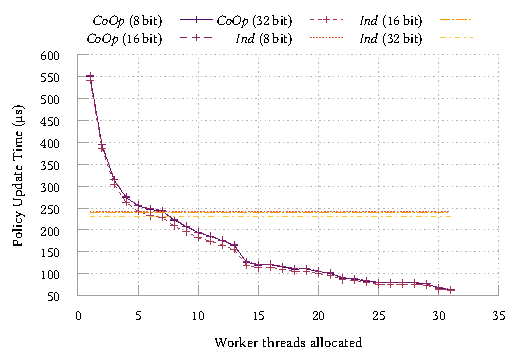
\includegraphics{../plots/build/rl-perf-tester/vary-core}
	}
	\caption{
		\Coopfw{}'s online learning performance improves as additional cores are made available, on max size tasks (\num{129} work items). This requires \num{8} workers to offer greater online throughput than single-threaded in-NIC RL. Sharper performance increases occur when a new physical core is added (\numrange{7}{8}) or the scheduler works around a bottleneck (\numrange{13}{14}).\label{fig:vary-core}}
\end{figure}

\begin{figure}
	\resizebox{0.9\linewidth}{!}{
		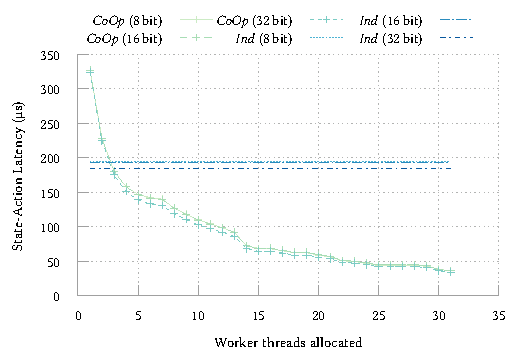
\includegraphics{../plots/build/rl-perf-tester/vary-core-latency}
	}
	\caption{\Coopfw{}'s action latencies improve with additional cores. This requires \num{3} workers (4 total contexts) to improve upon the state-action latency of single-threaded in-NIC RL.\label{fig:vary-core-latency}}
\end{figure}

\Cref{fig:vary-work,fig:vary-work-latency} show how policy complexity affects update costs and state-action latency respectively, scaling from a bias tile up to the full DDoS policy size\footnote{Input vectors here all have 20 elements regardless of the policy design.}.
\Coopfw{} always produces an action in less time than \Indfw{}, but requires at least one state-based tile to excel in online learning.
%We note that this is a trivial case, in that the use of \emph{only} a bias tile negates the need for any input state (similar to a multi-arm bandit problem).
We note that this is a trivial case, as using \emph{only} a bias tile returns a single preference list regardless of input state.

\begin{figure}
	\resizebox{0.9\linewidth}{!}{
		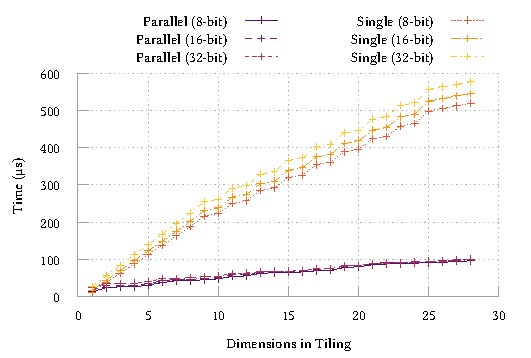
\includegraphics{../plots/build/rl-perf-tester/vary-work}
	}
	\caption{\Coopfw{} fully processes updates faster than \Indfw{}---thus has higher online performance---on almost all policy sizes. Lower bit depths are more effective on simpler policies.\label{fig:vary-work}}
\end{figure}

We found that a key aspect of in-NIC execution is that it allows far tighter bounds on tail latency compared to host offloading.
Examining the state-action latencies in \cref{tab:lats}, we see that \num{99.99}\nthscript{th} percentile latencies exceed the median by \SIlist{0.58;0.66}{\percent} for \Indfw{} and \Coopfw{}, respectively.
Similar results were observed for other bit depths.
By contrast, host-based tail latencies are at least \SI{40.53}{\percent} greater even when parallel workers are at or below the physical core count.
We show the cumulative distributions of these in detail (\cref{fig:lat-cumul}), noting how just one additional CPU-intensive task---potentially automated system updates, scans, or another vNF/traffic processing task---impacts tail latencies further (\emph{Float(Over)}).

\begin{figure}
	\resizebox{0.9\linewidth}{!}{
		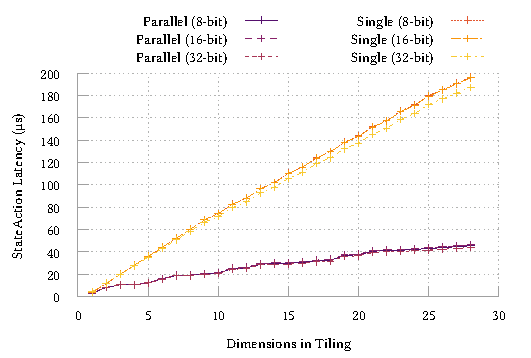
\includegraphics{../plots/build/rl-perf-tester/vary-work-latency}
	}
	\caption{State-action latency scales with additional work in a similar manner to overall processing time; though \SI{32}{\bit} firmwares become more effective sooner (at \num{3} work items).\label{fig:vary-work-latency}}
\end{figure}

\begin{figure}
	\centering
	\begin{subfigure}{0.45\linewidth}
		\resizebox{1.0\linewidth}{!}{
			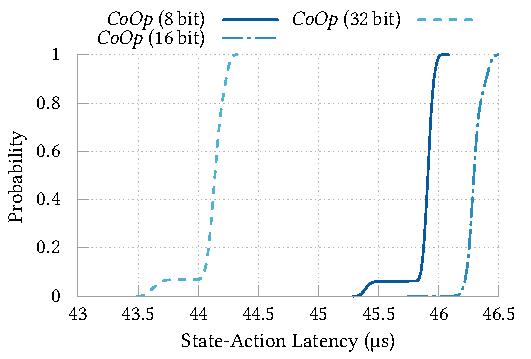
\includegraphics{../plots/build/rl-perf-tester/latency-cumul}
		}
		\caption{\approachshort's \Coopfw{} design achieves consistent, tight latency bounds.}
	\end{subfigure}
	\begin{subfigure}{0.45\linewidth}
		\resizebox{1.0\linewidth}{!}{
			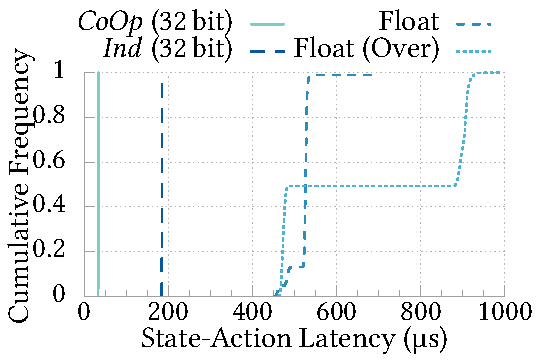
\includegraphics{../plots/build/rl-perf-tester/latency-cumul-broad}
		}
		\caption{Tail latencies suffer in host execution---particularly when oversubscribed.}
	\end{subfigure}
	\caption{Cumulative state-action latency plots for \approachshort{} and host-based execution.\label{fig:lat-cumul}}
\end{figure}

A noteworthy trend is that the \SIlist{8;16}{\bit} versions of \approachshort{} consistently underperform compared to \SI{32}{\bit} designs, with the exception of smaller workloads (seen in the zoomed portions of \cref{fig:vary-work,fig:vary-work-latency}).
This held even though our implementation is optimised to read and write policy tile data in batches (achieving fewer I/O operations as required).
This is due to the native register width on the NFP being \SI{32}{\bit}, and so the compiler must emit extra instructions around arithmetic operations to correctly load and update values.
This matches \SI{32}{\bit} becoming dominant in more complex workloads: higher dimension tilings require more arithmetic operations to compute the hit tile index.
Most of the I/O comes after this step, causing ALU use to dominate.
This also explains why \SI{32}{\bit} becomes the best choice at different policy complexities for online (\cref{fig:vary-work}, 10 dims) and offline (\cref{fig:vary-work-latency}, 3 dims) \Coopfw{} agents, where hashtable accesses and a \texttt{memcpy} of the state vector fall into the serial portion of the algorithm in the online case.
As a result, these bit depths give a \SIrange{2}{4}{$\times$} reduction in memory needed to store a policy (enabling more fine-grained or more complex policies), in exchange for slightly worse latency and throughput.
We investigated bit-stuffing several such values into a single word for our atomic writeback mechanism (as the platform offers both \SIlist{32;64
}{\bit} atomic addition).
This is analogous to SIMD---through clever use of padding bits---but we found that manipulating tiles into the correct format added \SI{10}{\percent} extra overhead.

\fakepara{Work allocation}
\Cref{fig:work-alloc-32} shows that our heuristic first-fit allocator (\emph{Balanced}) is key in achieving consistent sub-\SIlist{35;65}{\micro\second} latencies/processing times, respectively.
The trend is repeated for all bit depths, noting the latency differences described above.
The constant difference between \emph{Action} and \emph{Update Prep} was observed to scale linearly with bit depth, matching storage and lookup work in the serial portion between parallel jobs (plots omitted).
The severe underperformance of the \emph{Na\"{i}ve} allocator confirms that work item complexity is correlated with its ID, as batching work in contiguous chunks leads to some workers receiving exclusively high-dimensionality tile sets.
The minor gap in performance lower bounds between the \emph{Random} and \emph{Balanced} allocators suggests that further optimisations can be made in this way.
We expect that closing or exceeding this gap may require more complex modelling of NFP's hardware thread interactions, which lies far beyond the scope of in-NIC scheduling.
Some additional complexity may be tolerated, subject to code store limits---scheduling runs exactly once per configuration change, so does not impact per-action code.

\begin{figure}
	\resizebox{0.9\linewidth}{!}{
		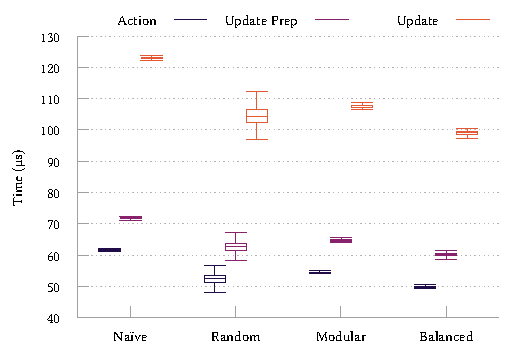
\includegraphics{../plots/build/rl-perf-tester/work-strat-32bit}
	}
	\caption{Action/update compute times in a \SI{32}{\bit} \Coopfw{} agent under different work schedulers.\label{fig:work-alloc-32}}
\end{figure}

\begin{figure}
	\resizebox{0.9\linewidth}{!}{
		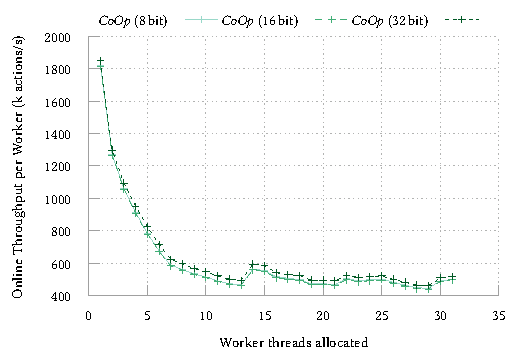
\includegraphics{../plots/build/rl-perf-tester/vary-core-tput-on-per}
	}
	\caption{Throughput per added worker in a \Coopfw{} agent.\label{fig:tput-per-core}}
\end{figure}

An interesting aspect of \Coopfw{} and the \emph{ParSa} algorithm in general is that adding cores has both diminishing returns and key thresholds to pass.
Consider \cref{fig:tput-per-core}, where the throughput per worker decreases over time but occasionally increases sharply.
Later downward ticks (\numrange{25}{29} workers) correspond to plateaus in throughput.
This is a problem stemming from the granularity of work items (i.e., tilings in \emph{ParSa}), where the heuristic scheduler cannot find a better solution to a bottleneck until extra cores are allocated.
We measured individual work items in state-action computation to take a mean \SIlist{5.2; 6.2; 9.7; 11.0}{\micro\second} for bias, CLS, CTM and IMEM tilings respectively.
While there is still a \SI{4.2}{$\times$} factor of task oversubscription at maximum worker count, it is clear that latencies are bound below by the length of the longest task.

\fakepara{End-to-end RL latency}
%?? PCIe RTT is 10us (neugebauer, BNN NFP paper), NFP RTT is 18us (own measurements). EMEM Ring one-way is 120ns.
%?? Cziva~\parencite[pp.113]{DBLP:phd/ethos/Cziva18} discusses vNF times.
%?? reference the inference times brought up in Taurus?
Referring to \cref{fig:state-slip}, we take $t_2$ from \cref{tab:lats} for host and in-NIC processing times, and substitute $t_1+t_3$ for the state packet round-trip time to the decision site:
\begin{description}
	\item[In-NIC.] As described in \cref{sec:agent-environment-communication}, EMEM rings have a median one way delay cross-island of \SI{140}{\nano\second}, giving a \emph{median \SI{34.63}{\micro\second} end-to-end inference latency}.
	\item[Dedicated Collector.] Offloads hosted in this manner will employ DPDK to maximise performance, giving one-way PCIe delays of \SIrange{0.9}{2.3}{\micro\second} for network packets.
	A UDP packet carrying \num{20} elements of state in \approachshort{} is \SI{128}{\byte}, so costs \SI{1}{\micro\second} to forward, and the reply state-action pair invokes a slightly higher cost.
	\emph{This gives an end-to-end inference latency of \SI{517.9}{\micro\second}}.
	\item[vNF Offload.] \Textcite{DBLP:journals/cm/CzivaP17} show that more lightweight vNF frameworks like GNF~\parencite{DBLP:journals/cm/CzivaP17} and ClickOS~\parencite{DBLP:conf/nsdi/MartinsAROHBH14} add \SIrange{45}{55}{\micro\second} \emph{additional} latency above PCIe costs.
	\emph{This gives an end-to-end inference latency of \SI{572.9}{\micro\second}}.
\end{description}
Using these estimates, in-NIC classical RL inference offers \SIlist{14.96;16.54}{$\times$} speedups in latency over collector and vNF deployments respectively (assuming no steering cost in either case).
We also contrast these against deep RL policies on network tasks, which can take \SI{3}{\milli\second} to compute~\parencite{DBLP:journals/corr/abs-1910-04054}---2 orders of magnitude above \approachshort{} with identically sized (20-dim) input vectors.
%In the name of fairness, we assume that rule installation uses same mechanism we recommend, but show how bad it can get? I.e. with rule installation costs etc.

\fakepara{Co-existence with the dataplane}
We were able to saturate the \SI{40}{\giga\bit\per\second} link for packet sizes at or above \SI{256}{\byte}.
%For frame sizes of \SIlist{64;128;256}{\byte} input traffic rates were \SIlist{17.4;32.9;37.0}{\giga\bit\per\second} respectively (\SIlist[per-symbol=p,sticky-per=true]{33.9;32.2;18.1}{\mega\packet\per\second}).
For frame sizes of \SIlist{64;128}{\byte} input traffic rates were \SIlist{17.4;32.9}{\giga\bit\per\second} respectively (\SIlist[per-symbol=p,sticky-per=true]{33.9;32.2}{\mega\packet\per\second}).
Passing this traffic over the loaded NFP device running \approachshort, no packet losses were incurred at any rate of RL actions.

We show the effect of RL workloads on the round-trip latencies of cross traffic through \cref{fig:dataplane-coop}.
As observed latency measures do not obey a normal distribution (particularly \SIlist{256;1518}{\byte}, which are bimodal), we employ a one-tailed \emph{Mann-Whitney U test} to mark statistically significant population increases in latency ($p < 0.05$) with a ``+''.
In general, we observe that statistically significant latency increases concentrate around smaller packet sizes.
All (bar one) of these affected \nth{99} percentile latencies by under \SI{0.38}{\percent} (at most \SI{78}{\nano\second}).
This slight degradation can be explained by increased pressure on the NFP's \emph{Command Push-Pull} (CPP) bus, which is responsible for handling cross-island accesses to memory (particularly IMEM/EMEM) and other resources.
\approachshort{} places load on the CPP bus through use of its \inring{}/\outring{} rings for external communication and through last-tier policy accesses.
This also explains the sensitivity of \SI{256}{\byte} packets to \approachshort{}---Netronome's P4 toolchain segments packets, storing metadata (e.g., MAC prepend data) and the first bytes of a packet in a $\SI{256}{\byte}$ CTM block and parking their payloads in EMEM.
\SI{256}{\byte} packets overshoot this due to metadata, causing small I/O accesses at a high rate for packets sized around this cutoff point.
Regardless, this effect is small when observed.

The anomalous result is \SI{128}{\byte} packets at \num{3000} RL action/update computations per second, causing a \SI{222}{\nano\second} (\SI{1.18}{\percent}) increase, shown in \cref{fig:dataplane-example}.
This is observed through a shift of some packet latencies from the mode towards the tail, but no other changes in the distribution.
In the above context, we believe that the inbound request rate is weakly synchronised with inbound packets, causing a higher level of burstiness around accesses to the CPP bus.
We expect that dedicated hardware/FPGA designs can avoid this problem by having dedicated \inring{}/\outring{} access mechanisms for an \approachshort{} agent.

\begin{figure}
	\centering
	\begin{subfigure}{0.45\linewidth}
		\resizebox{1.0\linewidth}{!}{
%			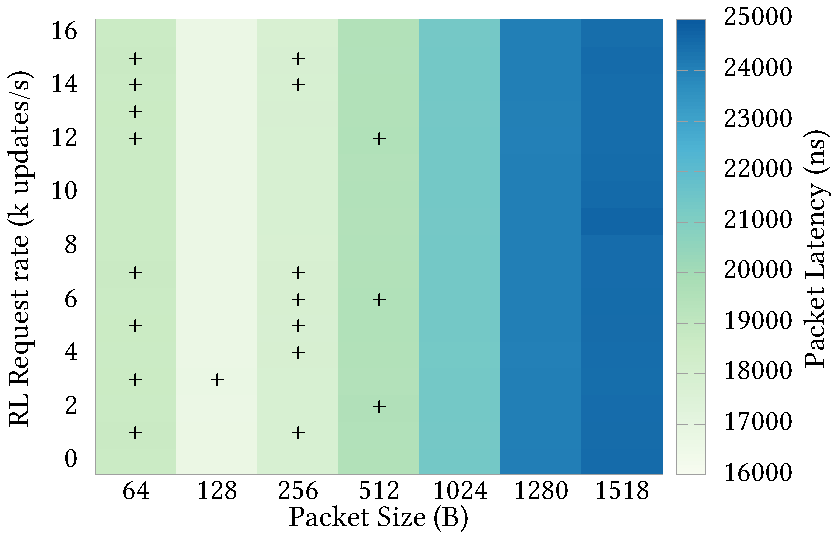
\includegraphics{../plots/build/stress/heat-latency-median}
			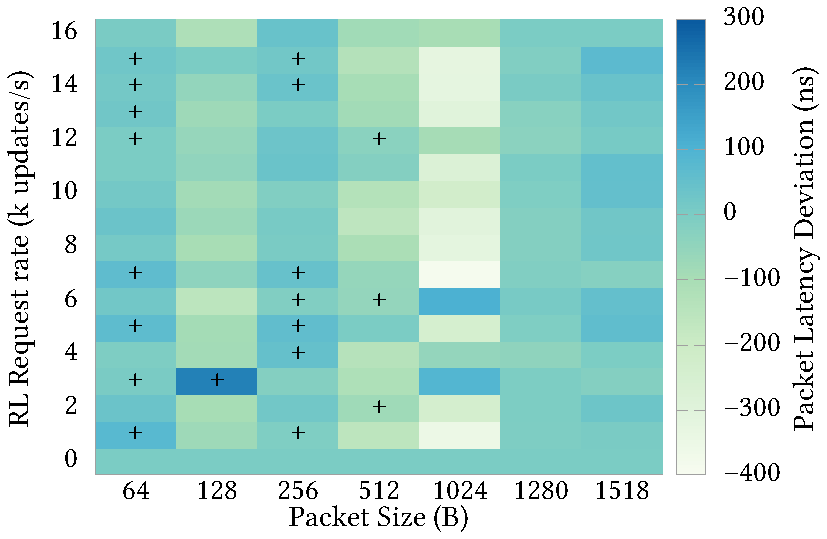
\includegraphics{../plots/build/stress/heat-latency-two-9-rel}
%			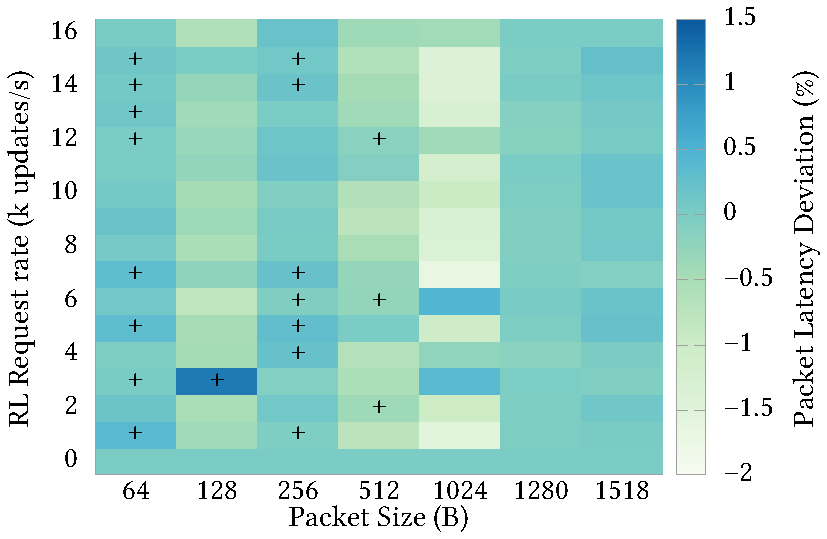
\includegraphics{../plots/build/stress/heat-latency-two-9-perc}
		}
		\caption{Deviations in \nth{99} percentile cross-traffic RTTs.\label{fig:dataplane-heat}}
	\end{subfigure}
	\hspace{0.05\linewidth}
		\begin{subfigure}{0.45\linewidth}
		\resizebox{1.0\linewidth}{!}{
			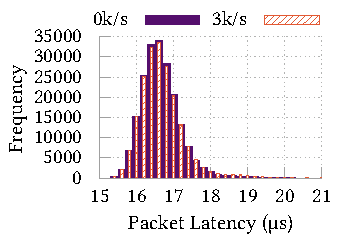
\includegraphics{../plots/build/stress/histo-128B-0-3-trim}
		}
		\caption{Distribution of RTTs for \SI{128}{\byte} packets for baseline and \num{3000} RL actions/s.\label{fig:dataplane-example}}
	\end{subfigure}
	\caption{Effects on tail latency of cross-traffic caused by different loads of off-path RL compute. Statistically significant increases in population latency are concentrated on smaller packet sizes, and are typically sub-\SI{78}{\nano\second}.\label{fig:dataplane-coop}}
\end{figure}

\fakepara{Resource requirements}
\Cref{tab:resources} demonstrates how \approachshort{} consumes shared and local memory as it scales to fit a device's compute resources, compared with a simple P4 forwarding application.
As one program is installed per ME, these results represent the minimum and maximum resource use we can command on a single island (i.e., without replacing P4 workers).
We observe negligible costs on shared bulk EMEM storage ($\sim$\SI{4}{\mebi\byte}), including storage space for a hash-table of \num{4096} state-action pairs and \num{16} reward values.
The most significant costs arise due to policy data (\SI{405}{\kibi\byte} shared IMEM, \SI{90}{\kibi\byte} local CTM, \SI{15}{\kibi\byte} local CLS), which can be halved or quartered using \SIlist{16;8}{\bit} quantisation and remain constant regardless of compute unit usage.
This causes a high upfront cost on per-island resources (CLS/CTM)---\approachshort{} leaves resources for other off-path dataplane applications, but is fairest from 3 cores onwards.

%Thread local storage in CLS for compute/register spilling scales with the number of MEs required (requiring \SIlist{13.77;15.49}{\percent} per-ME for \Indfw{}/\Coopfw) due to precaching and the space needed to hold tile lists.
%Due to the initial policy cost this falls below the fair share at 3 MEs, but always allows for co-existence with other asynchronous dataplane programs.

\begin{table}
\caption{NFP memory use due to \approachshort{} using \numlist{1;4} MEs (\SI{32}{\bit}). CLS and CTM regions are shared between all programs on the same island (placing our RL agent on i5), while EMEM and IMEM regions are shared between all NFP programs on a NIC.\label{tab:resources}}
\resizebox{\linewidth}{!}{
\begin{tabular}{
		@{}c
		S[table-format=4.2] S[table-format=2.2]
		S[table-format=4.2] S[table-format=2.2]
		S[table-format=4.2] S[table-format=2.2]
		S[table-format=2.2] S[table-format=2.2]
		S[table-format=3.2] S[table-format=2.2]
		@{}
	}
	\toprule Firmware & \multicolumn{2}{c}{EMEM} & \multicolumn{2}{c}{EMEM Cache} & \multicolumn{2}{c}{IMEM} & \multicolumn{2}{c}{i5.CLS} & \multicolumn{2}{c}{i5.CTM}\\
	& \multicolumn{1}{c}{\si{\mebi\byte}} & \multicolumn{1}{c}{\si{\percent}} & \multicolumn{1}{c}{\si{\kibi\byte}} & \multicolumn{1}{c}{\si{\percent}} & \multicolumn{1}{c}{\si{\kibi\byte}} & \multicolumn{1}{c}{\si{\percent}} & \multicolumn{1}{c}{\si{\kibi\byte}} & \multicolumn{1}{c}{\si{\percent}} & \multicolumn{1}{c}{\si{\kibi\byte}} & \multicolumn{1}{c}{\si{\percent}} \\
	\midrule Base P4 & 6776.67 & 88.24 & 268.52 & 2.91 & 858.28 & 10.48 & 0.00 & 0.00 & 0.00 & 0.00 \\
	\Indfw(1) & 6780.21 & 88.28 & 2541.08 & 27.57 & 1263.28 & 15.42 & 24.75 & 38.67 & 94.25 & 36.82 \\
	\Indfw(4) & 6780.22 & 88.28 & 2545.33 & 27.62 & 1263.28 & 15.42 & 51.18 & 79.97 & 107.00 & 41.80 \\
	\Coopfw(1) & 6779.12 & 88.27 & 1773.59 & 19.24 & 1263.28 & 15.42 & 22.41 & 35.01 & 90.00 & 35.16 \\
	\Coopfw(4) & 6779.12 & 88.27 & 1769.84 & 19.20 & 1263.28 & 15.42 & 52.16 & 81.49 & 90.00 & 35.16 \\
	\bottomrule
\end{tabular}
}
\end{table}

%\fakepara{The impact of bit depth}
%?? \Cref{fig:quant-acc}
%?? \SI{5}{\bit} mantissa suffices for $\ge$ \SI{90}{\percent} relative accuracy, so \SI{8}{\bit} is fine (1S + 2E + 5M), \SI{16}{\bit} is better.
%
%\begin{figure}
%	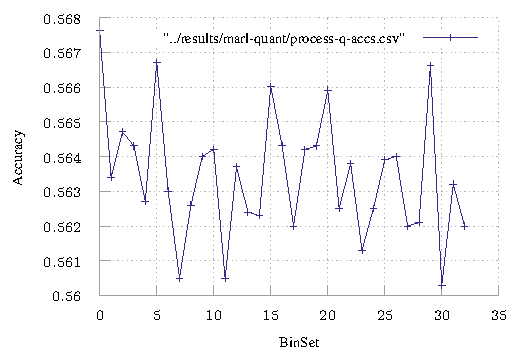
\includegraphics{../plots/build/marl-quant/accuracy-binary}
%	\caption{Normalised accuracy of a converted, pre-trained floating-point tile-coded policy after conversion to $32Qn$ fixed-point.}\label{fig:quant-acc}
%\end{figure}

\fakepara{Deployability}
Setup of \approachshort{} uses two packet types: \emph{setup} which contains learning (hyper-)parameters and most aspects of a tile coded policy, and \emph{tiling}, which provides a list of state indices for tiling sets.
We found that setup and tiling packets take a mean \qtylist{27.03;16.69}{\micro\second} to be processed on \Indfw{}, allowing for an agent to be swapped between online and offline operation (or repurposed for another task/policy) painlessly.
Online/offline swaps are useful when an agent should cease learning (i.e., when performance has converged to an acceptable value), or if a detected change in the environment means that more training is needed.
Tiling packet processing scales linearly with the number of \emph{tiling sets}, due to the needed precaching of tile set boundaries.
Online-offline swaps for \Coopfw{} exhibit similar cost, however the need for explicit ahead-of-time heuristic scheduling means that policy/tiling \emph{structure} changes (including the first complete setup) take \SI{422.63}{\micro\second} for the full-size policy described above.
The time taken for \Coopfw{} to schedule its tasks was found to scale with the number of workers ($m$) and work items ($n$) as described above ($\mathcal{O}{\left(n\log{m}\right)}$).
Ignoring the trivial solutions, reducing the worker count to \num{1} costs a mean \SI{238.22}{\micro\second}, while placing a single task incurs \SI{53.79}{\micro\second}.
Policy \emph{data} changes require no additional work in any case, resolving purely to \texttt{memcpy}s.

We observed that firmware installation (i.e., changing from \Indfw{} to \Coopfw{}, bit depth, or increasing maximum policy sizes) took a mean time of \SI{38.83}{\second}.
In the event that appropriate firmwares are not pre-compiled, we found that compiling and linking both \approachshort{} and the P4 toolchain took around \SI{35}{\second}, while changing only \approachshort{} parameters required around \SI{25}{\second}.
These results show that \approachshort{} can be easily adapted and altered by network administrators once in place, and illustrates an advantage of SoC-based SmartNICs.

\section{Potential Integrations}\label{sec:potential-integrations}
To show the general applicability and use of \approachshort{}, we propose an ideal integration which would benefit from in-NIC reinforcement learning; online DDoS attack mitigation.
We support this using other state-of-the-art P4/PDP developments, and discuss how best to balance the concerns of online training with throughput in widespread deployment.
Additionally, we discuss how network administrators may combine offline (\Indfw) and online (\Coopfw) agents within a network to achieve online learning while maximising action throughput in the majority of the network.

%?? How do we move this intuition to the start? ELI5 as dimitris says, to get the full end-to-end pipeline across to the reader.

\subsection{In-Network DDoS Defence}\label{sec:integ-1}
Classical RL has seen recent use in real-time, adaptive DDoS mitigation~\parencite{DBLP:journals/tnsm/SimpsonRP20}.
\Citeauthor{DBLP:journals/tnsm/SimpsonRP20}'s \emph{Guarded} agent design uses a mixture of global network state and local, per-flow state to monitor how flows respond to bandwidth changes and packet drop---applying the observations made by SPIFFY~\parencite{DBLP:conf/ndss/KangGS16} (observing how flow behaviour reacts to a change in rate limits) with more allowance for congestion-unaware protocols.
Actions then move flows up or down in punishment levels according to a finite state machine.

\fakepara{Why in-NIC?}
The above approach relies upon co-hosting traffic measurement and analysis alongside OpenFlow-compatible switches at the edge nodes of an AS.
However, packet mirroring, offloading RL computation to a host (potentially over layers of virtualisation), and CPU performance are all sources of additional, consistent state-action latency.
Both traffic statistics collection \emph{and} data-driven learning must be executed on such hosts/network functions.
Unless running these stages in a dedicated pipeline (adding further processing latency), resource contention between these processes will further impact tail latencies.
Naturally, this requires high-performance hardware to be stacked at network egress points, potentially beyond reasonable space, power, or ventilation constraints.
The solution to implement and improve upon this work using \approachshort{} is to place its RL agents on SmartNICs at AS edge nodes---a bump-in-the-wire deployment.

%?? Any way to move some of this sooner? I.e., this is ``why move DDoS prevention here'', Stefanos suggested backporting some of this to justify ``why \emph{RL} in-NIC''?

\fakepara{Inputs}
To collate the required inputs and state, we then examine the recent innovations of the community.
Low-latency, pure-P4 solutions to extract and record per-flow TCP state directly in the dataplane such as Dapper~\parencite{DBLP:conf/sosr/GhasemiBR17} and Sonata~\parencite{DBLP:conf/sigcomm/GuptaHCFRW18} are well-studied.
In fact, the statistics offered by Dapper are a super-set of the local input state values employed by \emph{Guarded} agents, offering an opportunity to further improve their efficacy. 
We propose placing such monitors in the P4 dataplane, existing on-chip alongside the \approachshort{} agent.
The required global state (load measures from network paths) must still come from elsewhere in the network; this is now the element at highest risk of becoming stale, but the least likely to vary significantly in response to individual actions.

The original work uses theoretical ``ground truth'' rewards, whose correct implementation and designs were left as an open challenge. 
We posit that INDDoS~\parencite{tnms-ddos-victim-ident}, which uses Count-min Sketches to estimate DDoS victim cardinality, could be an effective reward function source---i.e., using the number of detected victims as a loss value.

\fakepara{Integrating \approachshort}
Before each monitoring action, we require that the table hosting this hybrid solution polls \approachshort{}'s \emph{\outring{} Ring} for any generated actions.
As we note in \cref{sec:limitations}, these actions would be placed into a small hash table and simultaneously exported to the attached controller to be inserted as P4 rules in batches.
After the main monitoring step, packet ingress timestamps would be used to emulate the \emph{Timed Random Sequential} (TRS) scheduler used by the anti-DDoS agents for rate-controlled work, where state vectors would be selected and passed into \approachshort.
By design, active flows which are not \emph{judged} after a configurable time are discarded to prune the work set and allow new flows to be seen by the agent.
The tight bounds on execution time known \emph{a priori} make it easy to calculate the maximum number of decisions which can be made per deadline.
Reward values would then be separately inserted by a modified INDDoS table.

%?? Can I have a P4 code snippet here?

Reducing state-action latency (i.e., with \Coopfw) is useful for minimising the noise inherent in learning.
However, an agent is limited by the fact that it can take at least one RTT for meaningful changes to occur in a flow's behaviour ($\mathcal{O}{\left(\si{\milli\second}\right)}$ in a transit AS/ISP).
Accordingly, this use-case benefits most from an increase in \emph{throughput} using \Indfw{}.
In this context, higher throughput means that network flows are more likely to be judged in every timestep, even when flow cardinality is high---making it more likely that changes in flow behaviour will be observed, acted on, and learned from.

We note that the TRS scheduler is designed to handle cases where the number of flows created by an attacker is large, combining state vectors and information over time while the asynchronous agent is itself busy.
An increased number of (attack) flows beyond the maximum throughput simply makes it take longer in expectation for a flow to be reassessed.
As shown in \cref{sec:evaluation}, \approachshort{} far exceeds the throughput of host offloading.
The control plane is then free to use wildcards or specific matches to narrow down or expand the set of flows to be considered and controlled, though explicit scheduling techniques are still key in such adversarial environments.

%\subsection{Something host-specific?}\label{sec:integ-2}
%Accelerate something at an end-host... Flow control? Something datacentre-y? A novel CCA? What?

\subsection{Network Deployment Considerations}
The two compute models discussed above need not be homogeneously deployed.
For instance, in a networked deployment, a subset of \approachshort{} nodes could be \SI{32}{\bit} \coopfw{} agents, training online, while most other nodes run \SI{8}{\bit} \indfw{} designs to meet throughput guarantees.
The control plane would then be responsible for combining, downsampling, and distributing these improved policies between remaining agents.
This can be taken further still, using policy deltas or execution traces to enable out-of-path transfer learning for more complex function approximators such as neural networks.

\section{Related Work}
\fakepara{In-network ML}
Taurus~\parencite{DBLP:journals/corr/abs-2002-08987} proposes that efficient line-rate, low-latency per-packet inference can be achieved by placing a run-time configurable grid topology of map-reduce processing units into the packet processing pipeline (implementing CNNs, LSTMs, and some classical approaches such as SVMs).
Their CGRA-based implementation is able to be repurposed at runtime and achieves sub-\si{\micro\second} extra latency, though online model training is not considered.

\emph{IIsy}~\parencite{DBLP:conf/hotnets/XiongZ19} shows how \emph{classical ML inference} techniques (SVMs, Na\"{i}ve Bayes, Decision Trees, K-Means) can be converted into match-action table structures which are compatible with \emph{any} P4 deployment.
They achieve mean \SI{2.62}{\micro\second} extra in-path latency on NetFPGA devices (at line rate in most cases), but can only investigate the use of pre-trained models.

A recent line of research in the community has been to investigate \emph{Binarised/Bitwise Neural Networks} (BNNs)~\parencite{DBLP:conf/nips/HubaraCSEB16,DBLP:journals/corr/KimS16,DBLP:journals/corr/MiyashitaLM16} for line-rate, low latency packet classification.
\emph{BaNaNa SPLIT} shows the initial steps of this trend as an offload mechanism~\parencite{DBLP:conf/sigcomm/SanvitoSB18,DBLP:journals/corr/abs-1801-05731}; DNN inference is often carried out on the \emph{CPU} in an effort to reduce latency imposed by batching and bulk transfer to the GPU.
However, fully-connected layers are cache-unfriendly on commodity CPUs~\parencite{DBLP:conf/sigcomm/SanvitoSB18}, with the hypothesis put forward that networking hardware would be a better fit for some parts of the inference pipeline.
This line of work has moved onto full, in-network packet tagging and classification by pre-trained BNNs with \emph{N3IC}~\parencite{DBLP:journals/corr/abs-2009-02353}.
N3IC achieves packet inference in \SI{45}{\micro\second} on the NFP, and \SI{0.3}{\micro\second} on NetFPGA for \SI{256}{\bit} inputs.
Comparatively, \approachshort{}-\Coopfw{} can process an identically-sized input (8-dim) in a median \SI{13.83}{\micro\second}.
Our work handles larger inputs (\SI{640}{\bit}) at lower latencies of \SI{34}{\micro\second}, and offers online learning.
We expect that a NetFPGA implementation of \approachshort{} would enjoy a similar factor of speedup.
No works investigate the runtime training of BNN function approximators in-NIC.

\textcite{langlet-ml-netronome} has shown the viability of NN inference using \SI{64}{\bit} quantised weights and inputs on NFP hardware, using \emph{in-path} compute rather than our asynchronous model.
Inference latency on small networks (3 layers, \num{30} layers) can be as high as \SI{500}{\micro\second} on line rate traffic, stressing the value of the asynchronous compute and quantisation we adopt.

We note that none of the other approaches listed here (or that we have seen) tackle the issue of \emph{online learning and control} in-network---we believe \approachshort{} has broken new ground in this regard.

\fakepara{In-network ML \emph{acceleration}}
Optimisation of distributed neural network training is an area where in-network compute has been key for general NNs~\parencite{DBLP:conf/micro/LiPAYQPWSEK18} and RL-specific procedures~\parencite{DBLP:conf/isca/LiLYCSH19} using NetFPGAs to introduce floating point adders to process dedicated packet classes.
Distributed training is a partition-aggregate workload, where gradient vectors are sent back to a controller to update the `true' model---in-NIC processing allows these to be aggregated \emph{in-network}, overcoming incast behaviour and host bottlenecks.

\fakepara{RL for network control}
\Textcite{DBLP:conf/sigcomm/LiangZJS19} use deep RL techniques on a host machine to train an agent which can build efficient decision tree packet classifiers.
Their approach, \emph{NeuroCuts}, is able to produce time/space efficient classifiers for use in constrained environments (e.g., network hardware) beyond existing heuristic solutions.
Deep RL techniques have been used for QUIC congestion control optimisation~\parencite{DBLP:journals/corr/abs-1910-04054}.
A key facet of this work is the need for asynchronous RL in networks, where pauses for DNN-based inference can significantly harm throughput.

\fakepara{PDP design for asynchronous compute}
\Textcite{DBLP:conf/hotnets/StephensAS18} have proposed \emph{PANIC}, which places a routing fabric between distinct packet/data processing elements \emph{in a SmartNIC}.
Such designs would more generally enable asynchronous and novel compute in SmartNICs and programmable switches, for instance offering consistent and easy to use communication between workers versus hard-coded ME relationships.
Event-driven versions of the P4 pipeline have been suggested~\parencite{DBLP:conf/hotnets/IbanezABM19}.
Timer events and device state changes would empower in-network RL use-cases, signalling timesteps for RL agents or a new, effective, fine-grained sources of input state.

\section{Conclusion}
We have presented \emph{\approachshort{}}, bringing \emph{online reinforcement learning} to the dataplane.
\approachshort{} has shown how classical RL techniques make online learning possible by simplifying update logic and enable parallel processing.
These algorithms (and in-NIC deployment) enabled a \SIrange{15}{21}{$\times$} reduction in median--\num{99.99}\nthscript{th} inference times and order of magnitude improvement in online learning throughput compared to host offloading.
The deployment environment and asynchronous design were shown to eliminate PCIe and impose minimal impact on carried dataplane traffic.
\approachshort{}'s designs scale with additional compute resources at deployment to improve upon both decision latency and throughput.
Our throughput-optimal design, \Indfw{}, improves upon these metrics with \emph{just one worker}.

In future, we aim to examine the relative performance of individual applications driven by \approachshort---both classical and deep RL-based---and how a NetFPGA implementation can offer further latency and throughput improvements.
A promising avenue here would be to investigate constant transfer learning between a handful of online \approachshort{} agents and other high-throughput offline function approximators such as BNNs.
%It is our hope that high port-density programmable devices will, in time, expose similar asynchronous, on-chip offloading capability to current SmartNIC devices.
%We also are interested in `classical' approaches for other tasks which may have been overlooked in favour of more performant (yet complex) solutions, yet enable in-network deployment.

\begin{acks}
	The authors would like to thank Rhys Simpson for his comments, and for discussions on the soundness of SIMD-like optimisations.
	They would additionally like to thank Stefanos Sagkriotis, Mircea Iordache-\c{S}ic\u{a}, and Haruna Adoga for their comments and feedback.
	This work was supported in part by the \grantsponsor{gs-epsrc}{Engineering and Physical Sciences Research Council}{https://epsrc.ukri.org/} [grants~\grantnum{gs-epsrc}{EP/N509668/1}, \grantnum{gs-epsrc}{EP/N033957/1}].
\end{acks}
	
%\bibliographystyle{ACM-Reference-Format}
%\bibliography{reference}
\printbibliography

%\begin{appendices}
%	\section{Old ``What could we do''?}
%	How do we evaluate this without looking into classification performance?
%	\begin{itemize}
%		\item Analytically?
%		\begin{enumerate}
%			\item Prove that tile splitting scheme over memory hierarchy can improve performance.
%			\begin{itemize}
%				\item Hit rate of different tiles according to tile dimensionality?
%				\item Access time for each tier of memory hierarchy.
%			\end{itemize}
%		\end{enumerate}
%		\item Experimentally?
%		\begin{enumerate}
%			\item Create ``VNF'' testbed: mirror traffic from switch to a host for telemetry processing/flow state. Send flow state over to another node who computes RL actions. RL actions installed on switch.
%			\begin{itemize}
%				\item Why not co-host RL computation with telemetry? Could be separate functions, could want to ensure that neither impacts the performance of the other.
%			\end{itemize}
%			\item Create ``PDP'' testbed: Load firmware, pass in traffic. Traffic processing/action compute/table mod occurs in PDP.
%			\item What traffic? Healthy mix of attack (UDP), Discord legit Opus VoIP traffic, HTTP bulk-transfer traffic.
%			\item Measure $t_{1 \cdots 3}$ according to \cref{fig:state-slip} in both VNF and PDP contexts.
%			\begin{description}
%				\item[$t_1$]
%				\begin{description}
%					\item[PDP] Packet ingress $\rightarrow$ INT Island $\rightarrow$ State arrival in Control ME.
%					\item[VNF] Packet mirror time $\rightarrow$ telemetry VNF $\rightarrow$ state arrival in agent vnf.
%				\end{description}
%				
%				\item[$t_2$]
%				\begin{description}
%					\item[PDP] Time to compute action over parallel Policy MEs (RL Island, SmartNIC).
%					\item[VNF] Time to compute action in host program (on VNF) from received state.
%				\end{description}
%				
%				\item[$t_3$]
%				\begin{description}
%					\item[PDP] Modify local tables across ME/Island boundaries (same device), verify rule present (or get ACK).
%					\item[VNF] Generate OpenFlow control messages, send OF message to switch, verify rule present (or get ACK).
%				\end{description}
%			\end{description}
%			\item HYPOTHESIS: PDP will present a reduction in these three times for per-flow state.
%			\item QUESTION: Does same apply to learning?
%			\item NOTE: since we're not actually assessing the \emph{quality} of output decisions, we can cut corners on what data is sent out and where. I.e., in-band network telemetry island can be skipped, if we move over representative volumes of state to/from the RL island with approximately correct delay as recorded by other studies.
%		\end{enumerate}
%	\end{itemize}
%	I can think of one way to evaluate this if we employ classification performance:
%	\begin{enumerate}
%		\item Run the existing work~\parencite{DBLP:journals/tnsm/SimpsonRP20}, acquire a policy for one node after full info sharing.
%		\item Load this policy onto the RL Island (\cref{fig:netro-arch}).
%		\item Either feed in raw state packets, or feed in traffic if we can get INT working.
%		\item For each level of quantisation needed, examine average performance.
%		\item Don't compare against old numbers for final perf: use a ``VNF'' setup similar to above---this will probably suffer a bit compared to old results, where everything was on the same machine. Make it relative/normalised.
%	\end{enumerate}
%
%	\section{Intermediate steps?}
%	System?
%	\begin{itemize}
%		\item Setup other core as event source.
%		\begin{itemize}
%			\item \emph{\num{2} week.}
%			\item Idea: proxy for idea of INT core mentioned elsewhere, combined with the main periodic event sending that the last RL work relied upon. So, say "you can put that state management and extraction on another core, here's what the comms cost is" or similar.
%		\end{itemize}
%		\item Fixes to hash table use, signalling.
%		\begin{itemize}
%			\item \emph{\num{1} week.}
%			\item Blocks progress on optimisation, correct multi-stream RL.
%		\end{itemize}
%		\item Optimise/parallelise action compute/learning.
%		\begin{itemize}
%			\item \emph{\num{2} week.}
%			\item Value? Proves this approach can scale according to resource availability/demand on the deployment device, at compile-time anyhow.
%		\end{itemize}
%	\end{itemize}
%	
%	Experiments?
%	\begin{itemize}
%		\item Measure sum of times $t_{1...3}$ described elsewhere.
%		\begin{itemize}
%			\item \emph{\num{1} week.}
%			\item Currently have individual, need ``end-to-end''.
%		\end{itemize}
%		\item Throughput impact testing.
%		\begin{itemize}
%			\item \emph{\num{1} week.}
%			\item Requires current impl, creation of basic testbed and packet forwarding setup.
%			\item Use-case independent.
%		\end{itemize}
%		\item Measure execution, training costs for varying policy sizes.
%		\begin{itemize}
%			\item \emph{\num{1.5} weeks.}
%			\item Policies need not be meaningful, and can be garbage data. Use-case independent.
%			\item Partially blocked on multicore accelerated/optimised execution.
%		\end{itemize}
%		\item Measure rule installation cost on different platforms.
%		\begin{itemize}
%			\item \emph{\num{1.5} weeks.}
%			\item Blocked on creation of basic testbed and packet forwarding setup.
%		\end{itemize}
%		\item Investigate stationarity.
%		\begin{itemize}
%			\item \emph{\numrange{2}{3} weeks.}
%			\item Requires full use-case implementation.
%			\item Requires careful thought about sensible changes to normality.
%			\item Might be bolstered by comparison against an offline-trained system?
%		\end{itemize}
%	\end{itemize}
%	
%	\section{Everything we could possibly evaluate}
%	
%	Evaluation will need to be divided into 2 main categories:
%	\begin{enumerate}
%		\item Simulation/emulation based on mininet.
%		\begin{itemize}
%			\item These can only assess algorithmic properties, as performance measurements in mininet (i.e., a full mult-agent system) are not representative.
%		\end{itemize}
%		\item Testbed setup (2/3 configurations):
%		\begin{itemize}
%			\item These will assess key system performance properties of a \emph{single agent}, in control of a single switch/NIC as a bump in the wire. Bump-in-the-wire device will carry traffic between two hosts.
%			\item \emph{Time permitting, may need to send state vectors in packets rather than do feature/state extraction on-chip}.
%			\item \emph{Necessary.} RL runs on bump-in-the-wire SmartNIC.
%			\item \emph{Either/both.} P4-based off-path RL. Custom packet actions (e.g., random drop) will be implemented in P4 with externs. Packets/digests mirrored to state extraction machine. Agent may be co-hosted with state-extraction. Rules inserted via P4-device specific RTE.
%			\item \emph{Either/both.} OvS-based off-path RL. Custom packet actions are already implemented in OvS as OpenFlow extensions. Packets/digests mirrored to state extraction machine. Agent may be co-hosted with state-extraction.
%		\end{itemize}
%	\end{enumerate}
%	
%	\subsection{What is this different from, or better than?}
%	List below mainly for the benefit of helping enumerate everything I can compare against, and what their drawbacks are.
%	
%	\begin{itemize}
%		\item (Deep) neural network-backed RL.
%		\begin{itemize}
%			\item NNs infeasible to update online. Ordinarily this requires larger volumes of data than can be gathered in real time, but becomes substantially more difficult after change of representation (quantisation, binarisation). An online system (such as this) should be able to adapt to changes in underlying traffic, optimisation criteria, etc., dynamically.
%			\item Complexity of function approximation means that policy updates are more computationally complex to compute. For instance, NNs require use of the backpropagation algorithm, rather than the simpler classical schemes which need only the tile set already identified in action selection.
%			\item Only heavily quantised (i.e., binary neural networks) suitable for in-switch execution.
%		\end{itemize}
%		
%		\item MARL and other ``agents as network functions'' designs.
%		\begin{itemize}
%			\item Action, state collection, updates etc. happen on nodes outside of the main packet path in this paradigm. Thus, state measurements, action computation, and so on, should induce the state drift described above. Also makes these approaches ``slower to react'' in theory.
%		\end{itemize}
%	\end{itemize}
%	
%	At present, there are no other RL works in PDPs, let alone with online policy updates.
%	Other existing RL use cases suitable for adaptation to the ``bump-in-the-wire'' model are proving tricky to find.
%	
%	\subsection{Emulation metrics}
%	Key (MVP) metrics will be \textbf{bolded}, and expanded with a subsubsection.
%	
%	\textbf{Quantisation accuracy}, quantised training accuracy, \textbf{stationarity}.
%	
%	\subsubsection{Quantisation accuracy}
%	Examination of whether lower resolution quantisation impacts RL agent decision accuracy substantially.
%	
%	This has been done using MARL in mininet, see \cref{fig:quant-acc}.
%	
%	\subsubsection{Interaction with stationarity}
%	Learning time of the system as compared to known changes in normality.
%	
%	I.e., in the DDoS case: how long does an agent take to respond to the onset of an attack?
%	A change in attack strategy?
%	The conclusion of an attack?
%	There are no citations on \emph{how} DDoS attacks evolve, just that they do, and that this can occur on various timescales.
%	
%	\subsection{Testbed metrics}
%	Key (MVP) metrics will be \textbf{bolded}, and expanded with a subsubsection.
%	
%	\textbf{Traffic throughput (bytes, packets)}, \textbf{packet processing delay}, \textbf{action execution time}, \textbf{learning time}, from-scratch learning accuracy, \textbf{rule installation delay/cost}, host and NIC memory costs, policy installation time, ``accuracy'' in the DDoS case.
%	
%	\subsubsection{Traffic throughput}
%	Main research question: does moving RL logic onto the NIC reduce maximum throughput of the NIC, even if calculation is on a different functional unit?
%	This is relevant in both \si{\byte\per\second} and packets per second.
%	
%	This is application independent, and would assess whether the RL units (acting independently on the netronome) affect throughput compared with a basic P4 program at different work intensities.
%	Ideally, this would show no effect on forwarding performance.
%	
%	\subsubsection{Packet processing delay}
%	Main research question: does the presence of off-path (but on-chip) RL execution meaningfully increase packet processing delay? How does this compare to a P4 program with an equivalent number of tables? What about to OvS?
%	
%	\subsubsection{Action execution \& learning time}
%	Main research question: does moving RL logic from the host to the NIC substantially reduce delays from state measurement, to state receipt, to action computation and installation?
%	These constitute $t_{1...3}$ discussed above.
%	Primarily, these need to be looked at using varying policy sizes and distribution across memory regions.
%	
%	We ideally want these both with and without any acceleration from extra cores on the netronome: the point of this being that we can demonstrate that the system (or a similar NetFPGA system) can scale upwards according to available system resources or demands.
%	
%	\subsubsection{Rule installation delay/cost.}
%	Main research question: how long does it take to install rules in the above testbed setups? What is the downtime of so doing?
%	
%	This is application-dependent: see earlier discussions on rule batching and local extern/hash-table use.
%\end{appendices}

	
\end{document}